%% Paper 1 -- compile with:  latexmk -lualatex main.tex   (or Overleaf, compiler = LuaLaTeX)
\documentclass[preprint,12pt,authoryear,nonatbib]{elsarticle}
\usepackage{fontspec}
\setmainfont{Latin Modern Roman}
\usepackage{amsmath,amssymb}
\usepackage{graphicx,booktabs,tabularx,multirow,float}
\usepackage[margin=2.4cm]{geometry}
\usepackage{xcolor,enumitem,setspace}
\usepackage{tikz}
\usetikzlibrary{positioning,arrows.meta,fit}
\usepackage{xurl}
\usepackage[style=apa,backend=biber,sortcites=true]{biblatex}
\addbibresource{refs.bib}
\let\citep\parencite
\let\citet\textcite
\setlength{\bibhang}{0.5in}
\usepackage[hidelinks]{hyperref}
\usepackage{lineno}
\onehalfspacing
\setlength{\tabcolsep}{5pt}
\setlength{\emergencystretch}{2em}
\Urlmuskip=0mu plus 1mu
\newcommand{\tbd}[1]{\textcolor{red}{[#1]}}
\graphicspath{{figures/}}
\journal{Computers \& Education}

% Vietnamese abstract: keep for the HNUE conference version; set \vietnamesefalse for journal submission
\newif\ifvietnamese
\vietnamesetrue
\begin{document}
\begin{frontmatter}
\title{Connected but lonelier? A decade of digital transition and adolescent well-being in Viet Nam and East/Southeast Asia, 2012--2022}

\author[a]{\tbd{Author 1}\corref{cor1}}
\author[b]{\tbd{Author 2}}
\cortext[cor1]{Corresponding author: \tbd{email}}
\affiliation[a]{organization={\tbd{Affiliation 1}}, country={Viet Nam}}
\affiliation[b]{organization={\tbd{Affiliation 2}}, country={Viet Nam}}

\begin{abstract}
Between 2012 and 2022, home internet access among Vietnamese 15-year-olds rose from 29\% to 90\%, the fastest rise among ten East and Southeast Asian PISA systems. We combine four PISA cycles (250,587 students), school questionnaires, population indicators and phone-policy records to examine concurrent changes in well-being and achievement. Viet Nam retained paper-based assessment throughout. Mathematics anxiety met scalar invariance and increased by 0.33 SD; reported loneliness rose from 6.1\% to 14.4\%. Belonging failed scalar invariance: freeing all three negative-item intercepts attenuated its estimated latent decline from $-0.250$ to $-0.035$ SD, while partial invariance still failed. Item-specific exclusion trends should therefore not be read as a validated decline in general belonging. Five reweighting specifications did not assign the loneliness increase to measured home access, but cannot exclude unmeasured exposure or confounding. The adjusted home-computer mathematics association increased to 23 points. In 2022, the distraction--achievement association attenuated after conditioning on non-digital disorder; the distraction--anxiety association persisted in Viet Nam after multiple-testing correction. Phone bans were associated with less distraction ($-0.08$ SD), without statistically clear adjusted achievement or anxiety differences. School-grouped validation added regression calibration and a separate below-Level-2 classifier (Brier 0.164 versus 0.203 at baseline). These observational patterns are consistent with attention to school climate, connectedness and equity; they do not identify causal effects of digital access or phone policies.
\end{abstract}

\begin{keyword}
digital transition \sep adolescent well-being \sep loneliness \sep mathematics anxiety \sep digital distraction \sep PISA \sep measurement invariance \sep school phone policy
\end{keyword}
\end{frontmatter}

\ifvietnamese
\noindent\textbf{Tóm tắt.} Từ 2012 đến 2022, tỷ lệ học sinh 15 tuổi ở Việt Nam có internet tại nhà tăng từ 29\% lên 90\%, nhanh nhất trong 10 hệ thống giáo dục Đông Á và Đông Nam Á được khảo sát. Nghiên cứu kết hợp bốn chu kỳ PISA (250.587 học sinh), bảng hỏi nhà trường, chỉ số dân số và hồ sơ chính sách điện thoại. Lo âu toán học đạt bất biến đo lường cấp scalar và tăng 0,33 độ lệch chuẩn; tỷ lệ báo cáo cô đơn tăng từ 6,1\% lên 14,4\%. Tuy nhiên, thang đo thuộc về không đạt bất biến scalar: giải phóng intercept của cả ba mục phủ định làm mức giảm tiềm ẩn ước tính thu hẹp từ $-0,250$ xuống $-0,035$ độ lệch chuẩn, và mô hình partial-scalar vẫn không đạt tiêu chí bất biến. Vì vậy, xu hướng từng mục về cảm giác bị loại trừ không chứng minh mức suy giảm chung của cảm giác thuộc về. Năm cách tái trọng số không quy mức tăng cô đơn cho tiếp cận thiết bị tại nhà, nhưng không loại trừ tác động của hành vi sử dụng hay yếu tố gây nhiễu chưa đo. Chênh lệch điểm toán gắn với máy tính tại nhà tăng lên khoảng 23 điểm. Liên hệ giữa xao nhãng số và điểm toán thu hẹp khi kiểm soát mất trật tự phi kỹ thuật số; liên hệ với lo âu vẫn tồn tại ở Việt Nam sau hiệu chỉnh kiểm định bội. Cấm điện thoại gắn với ít xao nhãng hơn, nhưng chênh lệch điểm toán và lo âu sau điều chỉnh chưa rõ về mặt thống kê. Kiểm định chéo theo trường bổ sung đồ thị hiệu chuẩn và bộ phân loại riêng cho toán dưới mức 2 (Brier 0,164 so với 0,203 ở mô hình mốc). Đây là các mối liên hệ quan sát, không phải ước lượng tác động nhân quả của thiết bị hay chính sách.
\fi

\linenumbers
\section{Introduction}

Viet Nam's education system went online in a decade. Internet use in the population rose from 37\% in 2012 to 79\% in 2022 \citep{wdi2024}. National programmes such as \emph{Sóng và máy tính cho em} (``Connectivity and computers for students'') and pandemic-era remote schooling brought devices into most homes \citep{peer2024}. Vietnamese 15-year-olds have long outperformed what the country's income would predict in PISA \citep{dang2020}. Whether their well-being has kept pace with this transition is unknown. The question matters beyond Viet Nam: middle-income education systems across Asia are following the same path and are being urged to build ``smart, connected'' education ecosystems.

International research is divided on what digital transitions do to adolescents. One strand documents rising adolescent loneliness and falling achievement from around 2012 and links both to the spread of smartphones, largely through \emph{aggregate} trends \citep{twenge2021,twenge2025}. A second strand finds that \emph{individual-level} associations between technology use and well-being are small \citep{orben2019,przybylski2017} and have not grown over time \citep{vuorre2021}. The two positions are not necessarily contradictory. Societal digitalisation could change the social ecology of adolescence, with consequences for every student, even if a given student's own access matters little. Distinguishing these \emph{ecological} and \emph{individual-exposure} accounts requires data that combine trends with within-cohort associations, which most studies lack.

Classroom-level evidence is similarly mixed. Phone use during lessons impairs learning in experiments \citep{kuznekoff2013,mendoza2018}, and phone bans improved low achievers' scores in England \citep{beland2016}, but the ``brain drain'' effect of a phone's mere presence finds little meta-analytic support \citep{ward2017,bottger2023}. Policy has moved faster than evidence: a growing share of systems now restrict phones in schools \citep{unesco2023gem}. Viet Nam permits phones in class for learning purposes with the teacher's permission \citep{moet2020circular32}.

This study contributes in four ways. \textbf{First}, it provides a decade-long account with measurement tests of Vietnamese adolescents' well-being in the digital transition. It uses four PISA cycles in which, uniquely in the region, Viet Nam's administration mode never changed. \textbf{Second}, it tests the individual-exposure account directly, through within-cycle associations and a reweighting decomposition of the trend. \textbf{Third}, it separates digital distraction from general classroom disorder and links both to achievement and achievement emotions. \textbf{Fourth}, it combines student, school, system and policy data. School policies are evaluated with propensity-score weighting, and inference across 13 systems is corrected for multiple testing.

\section{Theoretical framework and hypotheses}

\paragraph{Displacement and the ecology of adolescence} The displacement hypothesis holds that time online crowds out face-to-face interaction and thereby erodes social connectedness \citep{kraut1998}. Applied to individuals, it predicts that students with more digital access report more loneliness. Applied to cohorts, it suggests that when connectivity becomes universal, the social environment of school itself changes. Peers are less available and attention is fragmented, which affects connected and less-connected students alike \citep{twenge2021}. The ``Goldilocks'' and specification-curve literature, by contrast, suggests that individual-level associations are small and non-linear \citep{przybylski2017,orben2019}. Belonging is a fundamental need \citep{baumeister1995} and a robust correlate of school functioning \citep{allen2018}, so changes in it are consequential either way.

\paragraph{Attention, disorder and achievement emotions} Digital distraction competes for the limited working memory needed for mathematics \citep{sweller1988}, but it also co-occurs with other forms of classroom disorder. Control-value theory \citep{pekrun2006} predicts that a classroom in which students cannot control their attention lowers perceived control over learning and therefore increases anxiety, even when the loss of instruction time is accounted for.

\paragraph{Self-regulation and school policy} Self-regulated learners manage their environment to protect attention \citep{zimmerman2002}. Turning off notifications is a concrete instance of this. School phone bans remove the stimulus rather than build the skill, and schools may adopt them in response to existing problems.

\paragraph{Hypotheses} \textbf{H1}: Between 2012 and 2022, indicators of social exclusion and mathematics anxiety among Vietnamese students increased. \textbf{H2 (individual exposure)}: within cycles, students with more home digital access report more loneliness and anxiety, and changes in access account for the trend. \textbf{H3}: digital distraction is associated with lower achievement and attenuates after conditioning on general classroom disorder. \textbf{H4}: digital distraction is associated with higher mathematics anxiety beyond classroom disorder and relationships. \textbf{H5}: school phone bans are associated with less distraction; digital self-regulation is associated with higher achievement. Figure~\ref{fig:framework} summarises the framework.

\begin{figure}[H]\centering
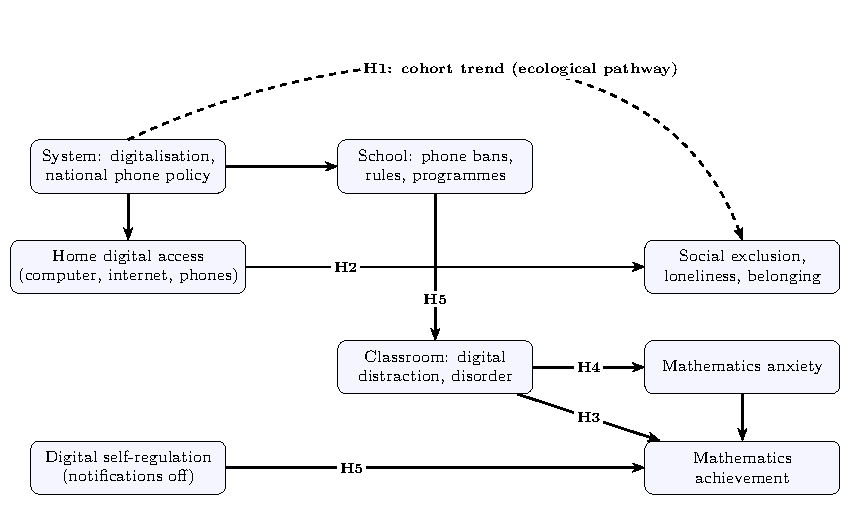
\includegraphics[width=\textwidth]{framework.pdf}
\caption{Conceptual framework and hypotheses. The dashed arrow is the ecological (cohort-level) pathway; solid arrows from home access are the individual-exposure pathway (H2). Arrows are hypothesised relationships, not identified causal effects.}\label{fig:framework}
\end{figure}

\section{Data}

Table~\ref{tab:sources} lists the five data sources. All are public and downloadable without registration.

\begin{table}[H]\centering\small
\caption{Data sources and levels of analysis}\label{tab:sources}
\begin{tabularx}{\textwidth}{@{}l>{\raggedright}p{3.9cm}lX@{}}
\toprule
\# & Source & Level & Content and use\\
\midrule
S1 & PISA 2012, 2015, 2018, 2022 student files \citep{oecd2022db} & Student & 250,587 students in 10 systems for trends (Viet Nam: 4,959; 5,826; 5,377; 6,068) and 88,087 students in 13 systems in 2022. Harmonised items on digital access, belonging, mathematics anxiety and classroom climate; digital distraction and digital habits (2022).\\
S2 & PISA 2022 school questionnaire & School & Principal reports on phone bans, rules on device use, responsible-internet programmes, SEL policy, school size, type and location.\\
S3 & World Bank WDI \citep{wdi2024} & System & Internet users, mobile subscriptions, GDP per capita, 2010--2023.\\
S4 & WHO Global Health Observatory \citep{whogho2025} & System & Suicide mortality (SDG 3.4.2), 2000--2021, used as population mental-health context.\\
S5 & UNESCO GEM PEER profiles \citep{peer2024} & Policy & National rules on phones in schools, coded with verbatim evidence.\\
\bottomrule
\end{tabularx}
\end{table}

\paragraph{Harmonisation} We use items with identical wording and response scales across cycles: computer for school work and internet at home (in 2022 the internet item excludes access through smartphones); three or more internet-enabled phones at home (2015--2022; 2022 categories mapped to the same threshold); the six sense-of-belonging items; five mathematics-anxiety items (2012 and 2022, the two cycles with mathematics as the main domain); and five mathematics disciplinary-climate items (2012 and 2022). We analyse raw item responses, not cycle-specific scaled indices, and we test their comparability directly (Section~\ref{sec:invariance}).

\paragraph{Administration mode} The other nine systems moved from paper-based to computer-based assessment in 2015 or 2018. Viet Nam remained paper-based in all four cycles (Appendix Table~\ref{tab:mode}), so Vietnamese trends are not confounded by changes in mode. Two data constraints are specific to Viet Nam. First, its 2018 performance data are not included in the public file, so 2018 contributes questionnaire indicators only. Second, the 2022 digital-habit items, which were part of the computer-based questionnaire only, are analysed for the eleven computer-based systems.

\section{Method}

\paragraph{Design-based estimation} Student-level descriptive and regression estimates use final student weights. Sampling variance uses 80 balanced repeated replication weights (Fay factor 0.5), and plausible-value variance (five in 2012, ten afterwards) is combined with Rubin's rules \citep{oecd2009manual,rubin1987}. Continuous predictors are standardised within system and cycle. Planned questionnaire rotation creates missingness by design; this does not make all item nonresponse missing completely at random. Regressions use complete cases on their variables, descriptive estimates use available responses, DFL uses missing-covariate categories, and LightGBM handles missing predictors natively. Complete-case associations require appropriate assumptions about response selection; analytic sample sizes are reported. Across-system hypothesis tests use false-discovery-rate correction \citep{benjamini1995}. CFA fit and machine-learning diagnostics are weighted descriptive estimates rather than BRR-adjusted hypothesis tests.

\paragraph{Measurement invariance}\label{sec:invariance} For Viet Nam we fitted one-factor multi-group confirmatory factor models to weighted item moments by maximum likelihood, separately for belonging (four cycles; residual covariances among the three negatively worded items to absorb the wording method effect) and mathematics anxiety (2012 vs 2022). We tested configural, metric and scalar invariance, applying the $\Delta\text{CFI} \geq -0.010$ criterion \citep{chen2007,putnick2016}, and estimated latent mean differences in units of the 2012 standard deviation.

\paragraph{Testing the individual-exposure account (H2)} Within each system and cycle, we regressed loneliness (linear probability, percentage points), the belonging scale and mathematics anxiety on home computer, internet and smartphones, controlling for ESCS, gender, grade, grade repetition and books at home. We then decomposed the 2012--2022 change in Viet Nam with DiNardo--Fortin--Lemieux reweighting \citep{dinardo1996}. The 2022 sample was reweighted to reproduce the 2012 distribution of (i) composition (gender, grade, repetition, books) and (ii) composition plus home computer and internet. The differences between the actual and counterfactual 2022 means give the parts of the change explained by composition and by access.

\paragraph{Digital distraction, 2022 (H3--H4)} DIGDIST is the mean of two items on distraction by one's own and by peers' digital devices in mathematics lessons. The official 2022 DISCLIM index contains these items, so we built a non-digital disciplinary-climate index from the five classic items. Models M1/M2 predict mathematics (background controls; + non-digital climate), and models A1/A2 predict mathematics anxiety (background controls; + climate, belonging, bullying, teacher support).

\paragraph{School policies (H5)} Phone bans are not randomly assigned. For each system we estimated school-level propensity scores for having a ban from school-mean ESCS, location, size and type, and applied stabilised inverse-probability weights \citep{rosenbaum1983}, with propensity probabilities clipped to .05/.95, in pooled models with system fixed effects and equal system weights.

\paragraph{Interpretable machine learning} LightGBM models \citep{ke2017} were trained per system and outcome. For performance, one model was trained for each plausible value; student weights were used and missing values were handled natively. Accuracy was assessed with five-fold cross-validation \emph{grouped by school}, against a weighted linear benchmark. Predictor importance is the weighted mean absolute SHAP value \citep{lundberg2017}. The same approach was applied by cycle with the harmonised features to track how the importance of predictors shifted over the decade.

\paragraph{Additional checks and calibration} We re-estimated belonging with B3 as the positive anchor, freeing the B1/B4/B6 intercepts across cycles, including a specification omitting 2018. Partial-scalar CFI is compared with the metric model, not with the already rejected full-scalar model. DFL sensitivity includes untrimmed weights, propensity clipping at .01/.99 and .05/.95, and density-ratio winsorisation at the 1st/99th and 5th/95th percentiles. Each stage is refitted with all 80 replicate weights separately for 2012 and 2022, summing independent-cycle variances. Weighted logistic fitting uses mean-one sampling weights to stabilise regularisation. A conditional permutation diagnostic jointly shuffles computer/internet labels 199 times within gender by ESCS-quintile strata; it is a model check, not a causal placebo. Reading is analysed as a comparison outcome rather than assumed to be unrelated to technology. For Viet Nam's 2022 LightGBM models we report weighted out-of-fold observed-on-predicted slopes, intercepts and decile reliability. A separate classifier for mathematics below Level 2 (420.07 points) reports weighted Brier scores against each fold's training-prevalence baseline \citep{oecd2023vol1}. All ten mathematics plausible values are fitted separately; target-missing cases are excluded. No validation fold contains schools from its training folds.

\section{Results}
Unless specified otherwise, descriptive tables use available-case final-weighted estimates, regression tables use model-specific complete cases and final weights, and parenthesised SEs use all 80 Fay BRR replicates (plus Rubin combination for achievement). Any stars denote $*p<.05$, $**p<.01$, $***p<.001$; $q$ denotes the Benjamini--Hochberg adjusted value. These conventions do not apply to CFA fit statistics, SHAP importance or prediction diagnostics. Table-specific sample sizes are unweighted counts.


\subsection{Are the measures comparable over time?}
Table~\ref{tab:invariance} reports the original invariance models. Mathematics anxiety met scalar invariance between 2012 and 2022 ($\Delta$CFI $= -0.009$; CFI $= 0.958$). Its RMSEA was elevated, as can occur with few degrees of freedom \citep{kenny2015}. The corresponding latent mean increased by \textbf{0.33 SD}. Belonging met metric invariance but failed scalar invariance. The targeted partial-scalar re-estimation freeing all three negative-item intercepts improves CFI from 0.749 to 0.916, but still falls 0.060 below the metric model (Table~\ref{tab:partial}). The 2022 latent contrast attenuates from $-0.250$ to $-0.035$ SD, or $-0.042$ SD when 2018 is omitted (Table~\ref{tab:partialmeans}). Thus the inference of a substantial common latent decline is sensitive to measurement assumptions; these failed-invariance estimates are diagnostic, not validated latent trends. Item-level changes remain informative (Table~\ref{tab:items}): negatively worded items move toward exclusion, while ``other students seem to like me'' increases. Complete item means, SDs and category frequencies are provided in Tables~\ref{tab:itemsB}--\ref{tab:itemsA}; response-style changes remain a plausible explanation.

\begin{table}[H]\centering\scriptsize
\caption{Measurement invariance, Viet Nam (multi-group CFA, ML on weighted moments)}\label{tab:invariance}
\begin{tabular}{@{}llrrrrr@{}}
\toprule
Scale (Viet Nam) & Model & $\chi^2$ & df & CFI & $\Delta$CFI & RMSEA \\
\midrule
Belonging & configural & 348.4 & 24 & 0.981 &  & 0.052 \\
Belonging & metric & 451.5 & 39 & 0.976 & -0.005 & 0.046 \\
Belonging & scalar & 4,417.1 & 54 & 0.749 & -0.227 & 0.127 \\
Belonging & partial scalar (free intercepts: B6) & 4,298.0 & 51 & 0.755 & +0.007 & 0.128 \\
Belonging & partial scalar (free intercepts: B5) & 3,123.1 & 51 & 0.823 & +0.074 & 0.109 \\
Belonging & partial scalar (free intercepts: B5, B2) & 2,702.1 & 48 & 0.847 & +0.098 & 0.105 \\
Belonging (excl. 2018) & configural & 222.2 & 18 & 0.985 &  & 0.048 \\
Belonging (excl. 2018) & metric & 298.7 & 28 & 0.980 & -0.005 & 0.044 \\
Belonging (excl. 2018) & scalar & 3,479.8 & 38 & 0.743 & -0.237 & 0.135 \\
Belonging (excl. 2018) & partial scalar (free intercepts: B6) & 3,439.8 & 36 & 0.746 & +0.003 & 0.138 \\
Belonging (excl. 2018) & partial scalar (free intercepts: B5) & 2,248.2 & 36 & 0.835 & +0.092 & 0.111 \\
Belonging (excl. 2018) & partial scalar (free intercepts: B5, B2) & 1,918.8 & 34 & 0.859 & +0.116 & 0.106 \\
Maths anxiety & configural & 631.1 & 10 & 0.967 &  & 0.117 \\
Maths anxiety & metric & 651.1 & 14 & 0.967 & -0.001 & 0.100 \\
Maths anxiety & scalar & 825.1 & 18 & 0.958 & -0.009 & 0.099 \\
\bottomrule
\end{tabular}

\par\smallskip\raggedright\footnotesize Final-weighted item moments; complete cases. Belonging models include residual covariances among B1/B4/B6. Here $\Delta$CFI is relative to the previous nested model, with earlier partial-scalar rows showing improvement over full scalar only; those positive differences do not establish invariance. The targeted partial-scalar check in Table~\ref{tab:partial} compares directly with metric. These ML fit statistics are not survey-adjusted tests.
\end{table}

\begin{table}[H]\centering\footnotesize
\caption{Viet Nam: belonging items, percentage giving the belonging response}\label{tab:items}
\begin{tabular}{@{}lrrrrr@{}}
\toprule
Item (\% giving the belonging response) & 2012 & 2015 & 2018 & 2022 & $\Delta$ 2012--22 \\
\midrule
Not an outsider (reversed) & 94.5 & 95.3 & 72.4 & 78.5 & -15.9 \\
Make friends easily & 92.0 & 91.6 & 80.0 & 85.4 & -6.6 \\
Feel I belong & 82.7 & 80.8 & 73.7 & 82.4 & -0.3 \\
Not awkward (reversed) & 88.8 & 82.7 & 76.7 & 70.5 & -18.2 \\
Other students like me & 40.8 & 42.6 & 36.9 & 65.1 & +24.3 \\
Not lonely (reversed) & 93.9 & 92.5 & 87.3 & 85.6 & -8.3 \\
\bottomrule
\end{tabular}

\end{table}

\subsection{A decade of change (H1)}
Table~\ref{tab:vnmtrend} and Figure~\ref{fig:trends} trace Viet Nam over the decade. Home internet access rose from 29.2\% to 89.6\%, and households with three or more smartphones rose from 29\% (2015) to 69\%, the fastest diffusion among the ten systems. The share of students who agreed that they feel lonely at school more than doubled (6.1\% to 14.4\%). Viet Nam began the decade as the least lonely system in the sample and recorded the largest increase (Table~\ref{tab:change}). Students who felt very tense doing mathematics homework rose from 33.3\% to 45.5\%, and those reporting noise and disorder in most mathematics lessons from 10.6\% to 17.6\%. Over the same period, disciplinary climate \emph{improved} in Korea, Malaysia, Chinese Taipei and Singapore (Figure~\ref{fig:dumbbell}). H1 is supported.

\begin{table}[H]\centering\footnotesize
\caption{Viet Nam, PISA 2012--2022: harmonised indicators (weighted; BRR standard errors in parentheses)}\label{tab:vnmtrend}
\begin{tabular}{@{}p{6.6cm}rrrr@{}}
\toprule
Indicator & 2012 & 2015 & 2018 & 2022 \\
\midrule
Students (N) & 4,959 & 5,826 & 5,377 & 6,068 \\
Mathematics mean (not a linked trend) & 511.3 (4.8) & 494.5 (4.5) & -- & 469.4 (3.9) \\
Socio-economic gradient (points per ESCS unit) & 29.4 (2.6) & 26.9 (3.2) & -- & 27.6 (2.2) \\
Gender gap, girls minus boys (points) & -9.9 & 3.0 & -- & -10.3 \\
Computer for school work at home (\%) & 39.6 (1.6) & 44.2 (1.5) & 41.6 (1.8) & 53.4 (1.7) \\
Internet at home (\%) & 29.2 (1.7) & 46.3 (1.5) & 76.9 (1.4) & 89.6 (0.8) \\
Three or more smartphones at home (\%) & -- & 29.1 (1.3) & 48.8 (1.6) & 69.4 (1.2) \\
`I feel like I belong at school' (\%) & 82.7 (0.8) & 80.8 (0.7) & 73.7 (0.9) & 82.4 (0.6) \\
`I feel lonely at school' (\%) & 6.1 (0.5) & 7.5 (0.6) & 12.7 (0.7) & 14.4 (0.5) \\
Sense of belonging, six items (1--4) & 3.02 (0.01) & 3.07 (0.01) & 2.81 (0.01) & 2.91 (0.01) \\
Mathematics anxiety, five items (1--4) & 2.54 (0.01) & -- & -- & 2.67 (0.01) \\
`I get very tense doing maths homework' (\%) & 33.3 (1.2) & -- & -- & 45.5 (0.9) \\
Disciplinary climate in maths (1--4, higher = better) & 3.25 (0.01) & -- & -- & 3.22 (0.01) \\
Noise and disorder in most/every maths lesson (\%) & 10.6 (0.8) & -- & -- & 17.6 (0.7) \\
\bottomrule
\end{tabular}

\par\smallskip\raggedright\footnotesize 2018 performance data for Viet Nam are not in the public file. Mathematics trends are descriptive (link error not added).
\end{table}

\begin{figure}[H]\centering
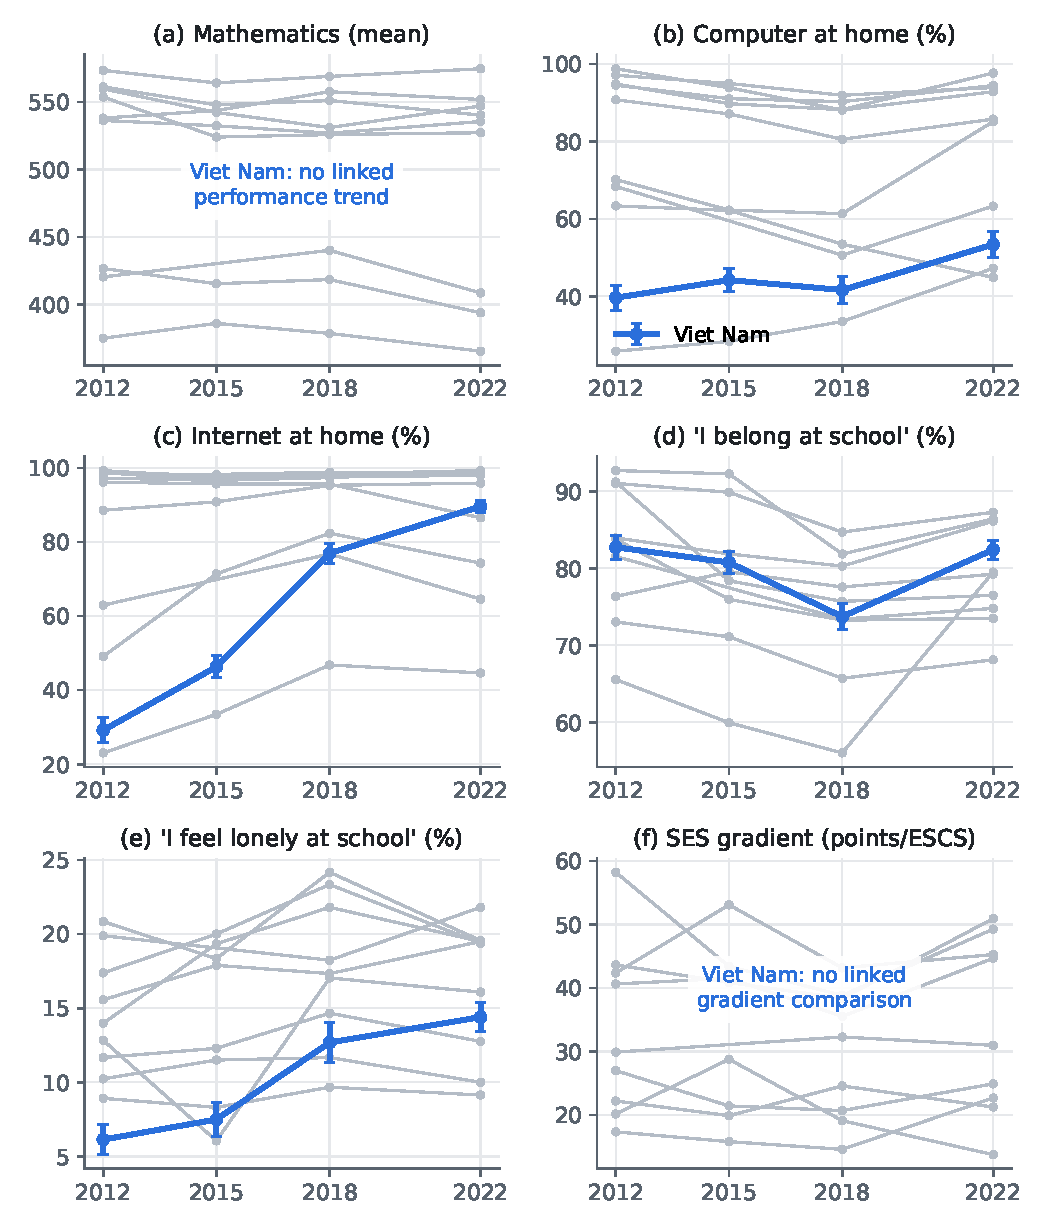
\includegraphics[width=\textwidth]{FigT1_trends_small_multiples.pdf}
\caption{Trends 2012--2022: (a) mathematics, (b) computer access, (c) internet access, (d) belonging agreement, (e) loneliness, (f) SES gradient. Viet Nam is blue with 95\% BRR intervals; nine other systems are grey. Total $n=250,587$; cycle-specific samples are in Table~\ref{tab:sources}. Available responses and final student weights are used.}\label{fig:trends}
\end{figure}

\begin{table}[H]\centering\footnotesize
\caption{Change 2012--2022 in harmonised indicators (percentage points unless stated)}\label{tab:change}
\begin{tabular}{@{}lrrrrrr@{}}
\toprule
 & Internet & Lonely & Belong & Maths anxiety & Tense & Noise \\
 & (pp) & (pp) & (pp) & (1--4) & (pp) & (pp) \\
\midrule
\textbf{Viet Nam} & +60.4*** & +8.3*** & -0.3 & +0.14*** & +12.2*** & +7.0*** \\
Singapore & +2.2*** & +3.9*** & -10.3*** & -0.04** & +0.1 & -5.5*** \\
Japan & +7.3*** & -0.2 & +2.2* & -0.01 & -1.3 & -4.9*** \\
Korea & +1.9*** & +0.2 & +2.9* & -0.22*** & -1.0 & -20.5*** \\
Chinese Taipei & -9.6*** & +1.1 & -3.7*** & -0.02 & +7.0*** & -8.5*** \\
Hong Kong (China) & -1.3*** & +5.5*** & -4.9*** & +0.09*** & +14.7*** & -4.0*** \\
Macao (China) & +0.3 & +2.0* & +14.0*** & +0.06*** & +2.0* & +2.1* \\
Thailand & +25.2*** & -1.3 & -14.7*** & -0.03 & +2.7 & -1.4 \\
Malaysia & +1.6 & +1.9 & -6.7*** & +0.08*** & +7.2*** & -12.4*** \\
Indonesia & +21.6*** & +3.3*** & -6.3*** & +0.16*** & +16.9*** & +6.1*** \\
\bottomrule
\end{tabular}

\par\smallskip\raggedright\footnotesize * $p<.05$, ** $p<.01$, *** $p<.001$ (independent samples, BRR standard errors).
\end{table}

\begin{figure}[H]\centering
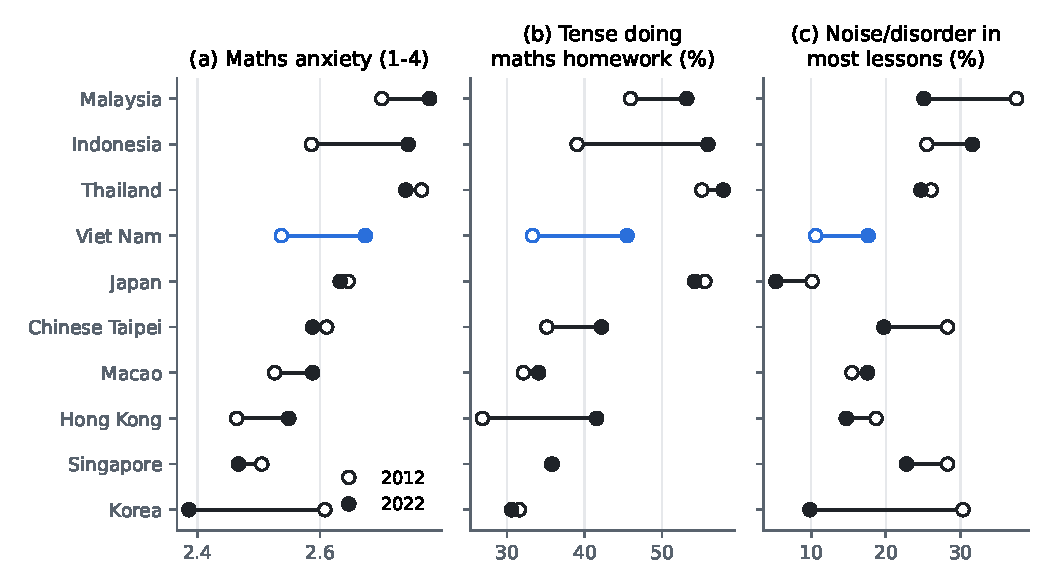
\includegraphics[width=\textwidth]{FigT2_dumbbell_2012_2022.pdf}
\caption{2012 (open) versus 2022 (filled): (a) anxiety, (b) homework tension, (c) classroom noise. Ten systems; available responses and final student weights. Cycle samples are in Table~\ref{tab:sources}; these panels show means without inferential intervals.}\label{fig:dumbbell}
\end{figure}

\subsection{Is the trend explained by students' own digital access? (H2)}
The measured home-access indicators provide little evidence for H2 in the adjusted within-cycle models (Table~\ref{tab:access}). Across the region, 91 system-cycle-indicator tests in the region, 25 significant at 5\%, all negative: where access mattered, it was associated with \emph{less} loneliness. In the updated DFL analysis, composition contributes $-0.61$ percentage points and access $-1.24$ points to the observed $+8.27$-point loneliness increase (Table~\ref{tab:dfl}). The access contribution remains non-positive across all five clipping specifications (Table~\ref{tab:dflsens}). The access-stage effective sample size is only 367 of 6,068 students with untrimmed weights, rising to 637 with .05/.95 probability clipping and 1,123 with 5th/95th-percentile ratio winsorisation (Table~\ref{tab:overlap}). Limited overlap therefore warrants caution despite stable point-estimate direction. These results do not support the proposed compositional explanation, but nonsignificance does not establish equivalence or exclude effects of usage intensity, content or unmeasured context. Conditional permutation diagnostics yield no unusual home-access coefficients under the selected null (Table~\ref{tab:perm}). Reading and mathematics are both positively associated with ICT resources in 2022 (17.76 and 18.17 points per SD; Table~\ref{tab:reading}); reading is therefore unsuitable as a technology-unrelated negative control.

Although measured digital access does not account for the well-being trend in this decomposition, its association with achievement has strengthened, raising an equity concern. This is an ancillary H2 finding; H5 concerns school phone policies and self-regulation rather than access inequality.

\begin{table}[H]\centering\scriptsize
\caption{Viet Nam: within-cycle associations of home digital access with well-being (SE in parentheses)}\label{tab:access}
\begin{tabular}{@{}llrrrr@{}}
\toprule
Outcome & Home access & 2012 & 2015 & 2018 & 2022 \\
\midrule
Lonely (pp) & Computer & -1.4 (1.5) & 0.7 (0.8) & -0.2 (1.2) & 0.6 (1.4) \\
Lonely (pp) & Internet & 0.6 (1.6) & 0.0 (0.9) & 0.1 (1.6) & -1.8 (1.9) \\
Lonely (pp) & Smartphone 3+ & -- & 1.4 (0.8) & -0.5 (1.2) & -1.7 (1.2) \\
Belonging (1--4) & Computer & 0.014 (0.024) & -0.020 (0.016) & 0.004 (0.014) & 0.029 (0.016) \\
Belonging (1--4) & Internet & 0.029 (0.027) & 0.020 (0.018) & 0.017 (0.023) & 0.050 (0.026) \\
Belonging (1--4) & Smartphone 3+ & -- & -0.006 (0.015) & 0.020 (0.015) & 0.025 (0.015) \\
Maths anxiety (1--4) & Computer & -0.018 (0.027) & -- & -- & 0.005 (0.028) \\
Maths anxiety (1--4) & Internet & -0.040 (0.029) & -- & -- & 0.017 (0.034) \\
Maths anxiety (1--4) & Smartphone 3+ & -- & -- & -- & 0.015 (0.021) \\
\bottomrule
\end{tabular}

\par\smallskip\raggedright\footnotesize Controls: ESCS, gender, grade, grade repetition, books at home. Lonely: percentage points; belonging and anxiety: scale points (1--4).
\end{table}

\begin{table}[H]\centering\footnotesize
\caption{Viet Nam: DiNardo--Fortin--Lemieux decomposition of the 2012--2022 change}\label{tab:dfl}
\begin{tabular}{@{}lrrrr@{}}
\toprule
Outcome & Change & Composition & Access & Residual\\
\midrule
Loneliness (pp) & 8.27 (0.72) & -0.61 (0.42) & -1.24 (1.77) & 10.12 (2.00)\\
Belonging (1--4) & -0.11 (0.01) & -0.00 (0.01) & 0.05 (0.03) & -0.16 (0.03)\\
Anxiety (1--4) & 0.14 (0.02) & -0.00 (0.01) & 0.01 (0.03) & 0.13 (0.03)\\
Tension (pp) & 12.18 (1.55) & -0.52 (0.51) & -0.50 (2.15) & 13.20 (2.53)\\
Noise (pp) & 7.03 (1.09) & -0.56 (0.45) & 1.52 (1.99) & 6.07 (2.29)\\
\bottomrule
\end{tabular}

\par\smallskip\raggedright\footnotesize SE in parentheses; final student weights with untrimmed DFL ratios. Composition: gender, grade, repetition, books; access: computer/internet. Available outcomes; missing covariates form categories. All 80 Fay BRR replicates are refitted independently in each cycle. Residual = change not accounted for by measured composition/access, not an identified causal mechanism. Full sample and weight diagnostics accompany the code.
\end{table}

\paragraph{Access and achievement inequality} Although measured access did not account for the well-being trend, its adjusted association with achievement strengthened (Table~\ref{tab:vnmrel}). In 2012 a home computer was unrelated to mathematics net of ESCS and books ($-4.9$, n.s.); by 2022 it was associated with $+23.4$ points. In the machine-learning models (Figure~\ref{fig:shapcycle}), the share of predictive importance attributable to a home computer rose from 2\% to 14\% and to smartphones from 4\% to 10\%, while grade level, a marker of late entry and repetition, fell from 32\% to 8\%.

\begin{table}[H]\centering\footnotesize
\caption{Viet Nam: changing relationships with mathematics performance (points; SE in parentheses)}\label{tab:vnmrel}
\begin{tabular}{@{}lrrr@{}}
\toprule
Predictor of mathematics & 2012 & 2015 & 2022 \\
\midrule
Computer at home (vs none) & -4.9 (3.8) & 10.5** (4.0) & 23.4*** (3.4) \\
Internet at home (vs none) & 23.8*** (4.7) & 12.6** (4.0) & 27.5*** (5.4) \\
Sense of belonging (per SD) & 4.6* (2.0) & -2.8 (1.7) & 4.9*** (1.2) \\
Mathematics anxiety (per SD) & -25.1*** (2.0) & -- & -14.2*** (1.3) \\
\bottomrule
\end{tabular}

\par\smallskip\raggedright\footnotesize Computer and internet models control for ESCS, gender and books; belonging and anxiety models for ESCS and gender.
\end{table}

\begin{figure}[H]\centering
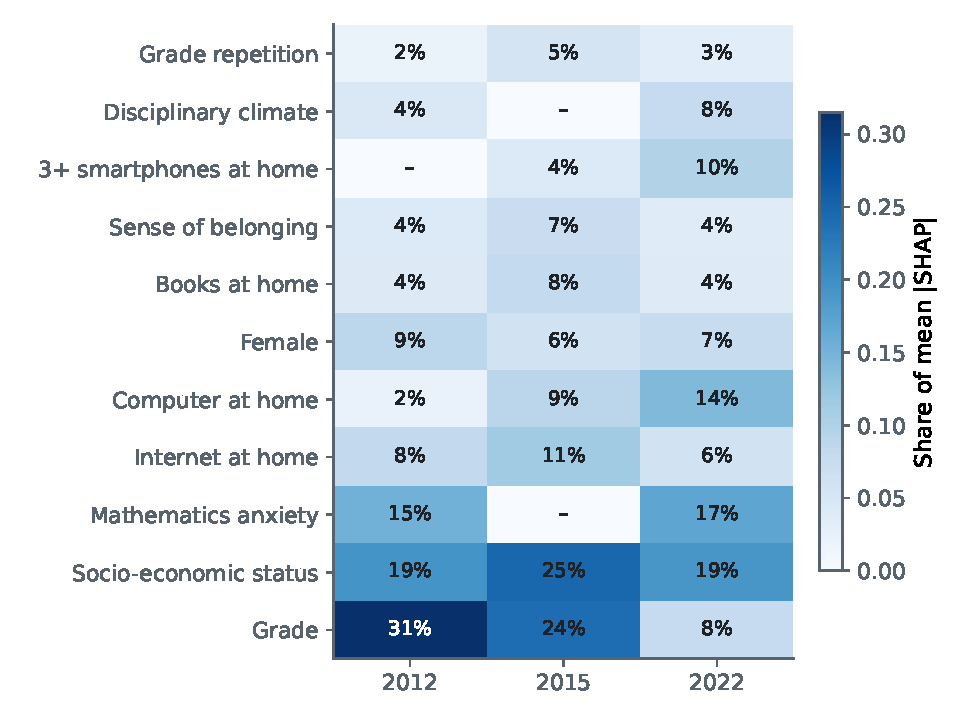
\includegraphics[width=.92\textwidth]{FigT3_vnm_shap_by_cycle.pdf}
\caption{Viet Nam: share of SHAP importance of harmonised predictors of mathematics, by cycle (school-grouped CV $R^2$ = 0.36, 0.21, 0.23; $n=4,959$, 5,826 and 6,068 in 2012, 2015 and 2022). Final-weighted LightGBM fits use native missing-predictor handling; SHAP shares describe prediction, not causal importance.}\label{fig:shapcycle}
\end{figure}

\subsection{Digital distraction in 2022 (H3, H4)}
In 2022, 14.3\% of Vietnamese students reported digital distraction in most or every mathematics lesson, compared with 5.2\% in Japan and 40.9\% in the Philippines (Table~\ref{tab:desc22}, Figure~\ref{fig:prev}). With background controls, distraction predicted lower mathematics scores in 12 of 13 systems (Viet Nam $-4.1$ points per SD). After non-digital disorder was controlled, the association disappeared in Viet Nam ($+0.7$) and was significant in only 6 of 13 systems after false-discovery-rate correction (Table~\ref{tab:models22}, Figure~\ref{fig:forest}). H3 is supported. Distraction predicted mathematics anxiety with background controls in 9 of 10 systems. After controlling for climate, belonging, bullying and teacher support, \textbf{Viet Nam was the only system} in which the association remained significant after correction ($+0.08$ SD, $q<.001$; Figure~\ref{fig:forestanx}). The SHAP dependence curve shows that it is concentrated among students who are distracted in every lesson (Figure~\ref{fig:dep}). H4 is supported for Viet Nam. In the eleven computer-based systems, students who turned off notifications in class scored 9--20 points higher per SD in 10 of 11 systems (Figure~\ref{fig:habits}).

\begin{table}[H]\centering\scriptsize
\caption{Digital distraction, digital habits, mathematics and anxiety, PISA 2022}\label{tab:desc22}
\begin{tabular}{@{}lrrrrrrr@{}}
\toprule
System & $N$ & \multicolumn{2}{c}{Distracted, most lessons (\%)} & Online & Nervous & Maths & ANXMAT \\
 & & own devices & peers' devices & pressure (\%) & w/o device (\%) & &  \\
\midrule
\textbf{Viet Nam} & 6,068 & 14.2 (0.7) & 12.7 & -- & -- & 469.4 (3.9) & 0.45 \\
Singapore & 6,606 & 27.3 (1.1) & 20.6 & 11.6 & 16.3 & 574.7 (1.2) & 0.15 \\
Japan & 5,760 & 5.2 (0.5) & 3.9 & 4.0 & 17.0 & 535.6 (2.9) & 0.33 \\
Korea & 6,454 & 9.4 (0.6) & 8.8 & 24.5 & 10.0 & 527.3 (3.9) & -0.05 \\
Chinese Taipei & 5,857 & 15.9 (1.0) & 12.5 & 21.9 & 14.1 & 547.1 (3.8) & 0.29 \\
Hong Kong (China) & 5,907 & 16.4 (0.9) & 15.2 & 19.3 & 20.5 & 540.4 (3.0) & 0.23 \\
Macao (China) & 4,384 & 13.3 (0.7) & 11.6 & 23.1 & 23.6 & 551.9 (1.1) & 0.28 \\
Thailand & 8,495 & 26.4 (0.9) & 22.9 & 10.9 & 21.7 & 393.9 (2.7) & -- \\
Malaysia & 7,069 & 20.3 (1.0) & 19.0 & 16.3 & 27.1 & 408.7 (2.4) & 0.50 \\
Indonesia & 13,439 & 25.1 (0.9) & 26.6 & 15.8 & 35.1 & 365.5 (2.4) & -- \\
Philippines & 7,193 & 40.9 (0.9) & 37.5 & 29.7 & 23.9 & 354.7 (2.6) & -- \\
Brunei Darussalam & 5,576 & 11.5 (0.4) & 10.5 & 23.6 & 25.6 & 442.1 (0.9) & 0.67 \\
Cambodia & 5,279 & 19.2 (0.8) & 20.8 & -- & -- & 336.4 (2.7) & 0.50 \\
\bottomrule
\end{tabular}

\par\smallskip\raggedright\footnotesize ``--'': not administered (paper-based systems or national option).
\end{table}

\begin{figure}[H]\centering
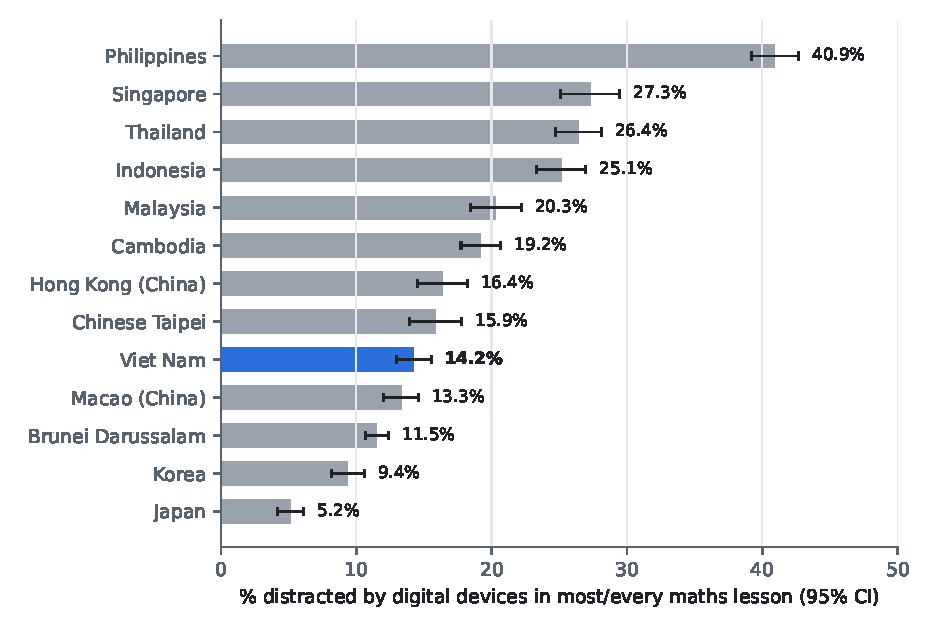
\includegraphics[width=\textwidth]{Fig1_prevalence_digital_distraction.pdf}
\caption{Students distracted by digital devices in most or every mathematics lesson: final-weighted percentages with 95\% BRR intervals. Thirteen systems, base $n=88,087$; percentages exclude missing item responses.}\label{fig:prev}
\end{figure}

\begin{table}[H]\centering\footnotesize
\caption{Digital distraction (DIGDIST) coefficients, PISA 2022 (SE in parentheses)}\label{tab:models22}
\begin{tabular}{@{}lrrrr@{}}
\toprule
 & \multicolumn{2}{c}{Mathematics (points per SD)} & \multicolumn{2}{c}{Maths anxiety (index per SD)} \\
System & M1 & M2 (+climate) & A1 & A2 (+climate, relations) \\
\midrule
\textbf{Viet Nam} & -4.1* (1.9) & 0.7 (2.3) & 0.20*** (0.02) & 0.08*** (0.02) \\
Singapore & -9.9*** (2.1) & 0.9 (2.3) & 0.11*** (0.02) & 0.01 (0.02) \\
Japan & -7.4** (2.5) & 1.1 (2.3) & 0.09** (0.03) & 0.00 (0.03) \\
Korea & -6.0** (2.1) & -7.6** (2.4) & 0.08** (0.03) & 0.03 (0.03) \\
Chinese Taipei & 0.8 (3.3) & 5.1 (3.9) & 0.09** (0.03) & 0.03 (0.03) \\
Hong Kong (China) & -10.7*** (2.8) & -3.8 (3.2) & 0.13*** (0.03) & 0.06* (0.03) \\
Macao (China) & -13.1*** (1.8) & -11.0*** (2.0) & 0.06* (0.02) & -0.02 (0.03) \\
Thailand & -6.9*** (1.6) & 2.3 (2.2) & -- & -- \\
Malaysia & -16.8*** (1.5) & -8.9*** (1.7) & 0.05* (0.02) & -0.04 (0.03) \\
Indonesia & -6.5*** (1.4) & -3.1 (1.8) & -- & -- \\
Philippines & -5.8*** (1.2) & 3.6** (1.2) & -- & -- \\
Brunei Darussalam & -13.6*** (1.8) & -7.3*** (1.8) & 0.03 (0.02) & -0.00 (0.02) \\
Cambodia & -8.8*** (1.4) & -7.4*** (1.7) & 0.15*** (0.01) & 0.04* (0.02) \\
\bottomrule
\end{tabular}

\par\smallskip\raggedright\footnotesize Controls: ESCS, gender, grade, grade repetition. * $p<.05$, ** $p<.01$, *** $p<.001$ (unadjusted). Benjamini--Hochberg significant at $q<.05$: M1: 12/13; M2: 6/13; A1: 9/10; A2: 1/10.
\end{table}

\begin{figure}[H]\centering
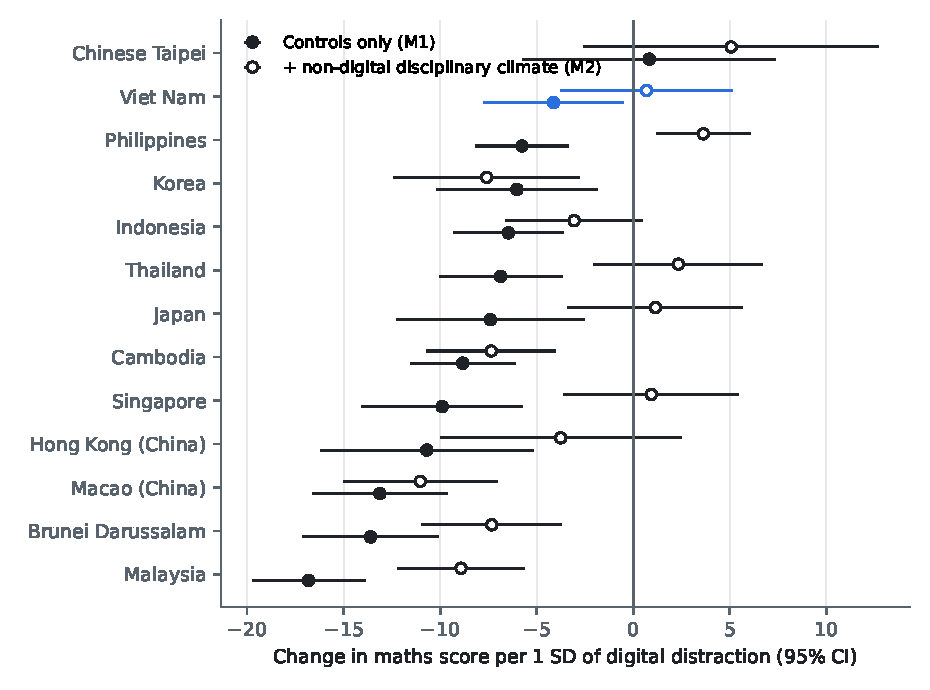
\includegraphics[width=.95\textwidth]{Fig2_forest_math.pdf}
\caption{Digital distraction and mathematics before (M1) and after (M2) conditioning on non-digital disorder. Dots: coefficients; bars: 95\% BRR/Rubin intervals using ten plausible values, final weights and complete cases. Thirteen systems; system sample sizes are in Table~\ref{tab:modeln}.}\label{fig:forest}
\end{figure}

\begin{figure}[H]\centering
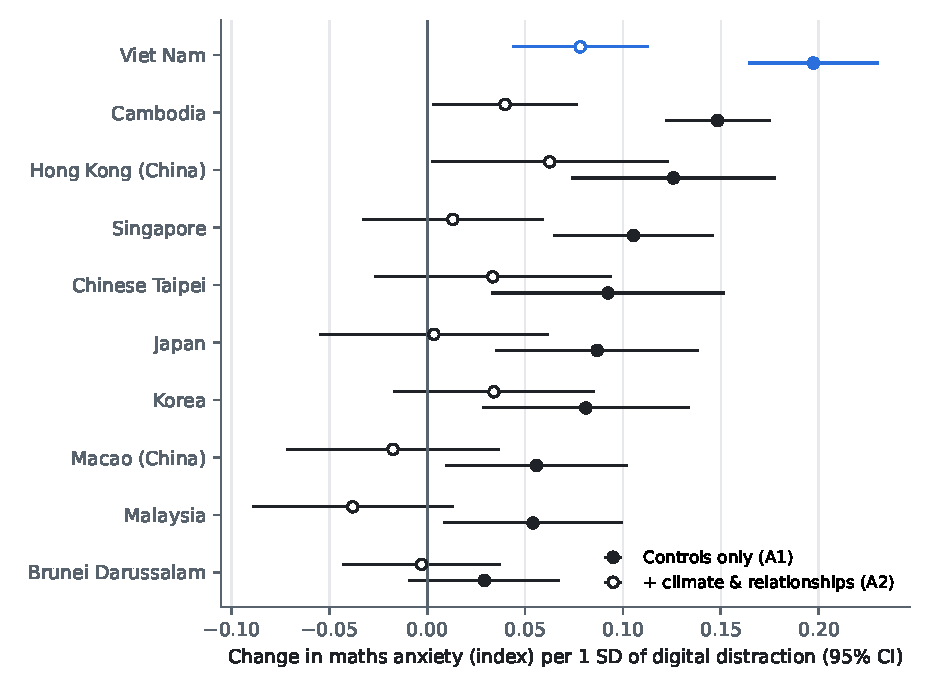
\includegraphics[width=.95\textwidth]{Fig3_forest_anxiety.pdf}
\caption{Digital distraction and mathematics anxiety before (A1) and after (A2) controls. Dots: coefficients; bars: 95\% BRR intervals using final weights and complete cases. Ten systems; model sample sizes are in Table~\ref{tab:modeln}.}\label{fig:forestanx}
\end{figure}

\begin{figure}[H]\centering
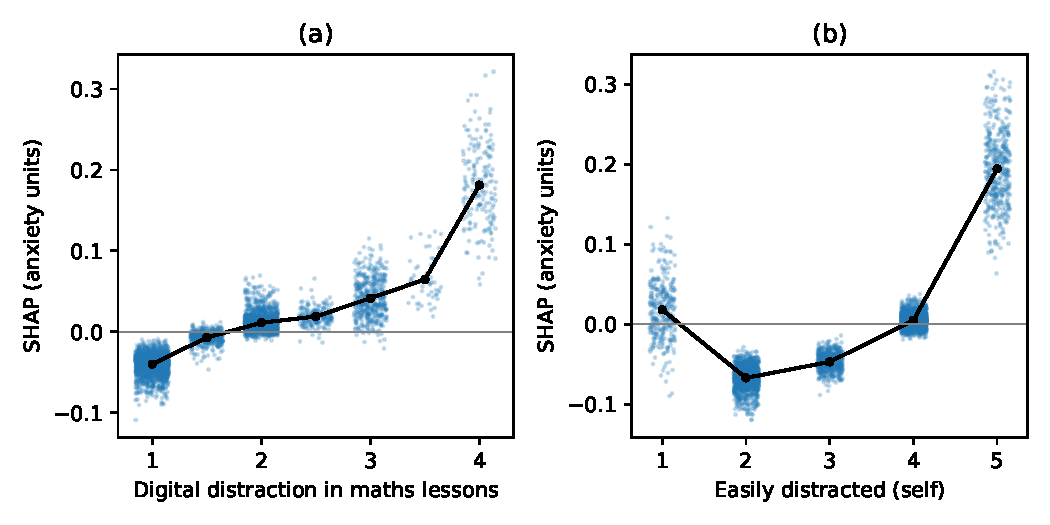
\includegraphics[width=.95\textwidth]{F_shap_dependence_VNM_ANXMAT.pdf}
\caption{Viet Nam: SHAP dependence of mathematics anxiety on (a) digital distraction in mathematics lessons (1 = never, 4 = every lesson) and (b) ``I get easily distracted'' (1 = strongly disagree, 5 = strongly agree). Black line: unweighted mean SHAP value per response level; $n=5,934$ Vietnamese students with observed anxiety. The fitted LightGBM model uses final student weights; this is a predictive dependence plot, not a causal contrast.}\label{fig:dep}
\end{figure}

\begin{figure}[H]\centering
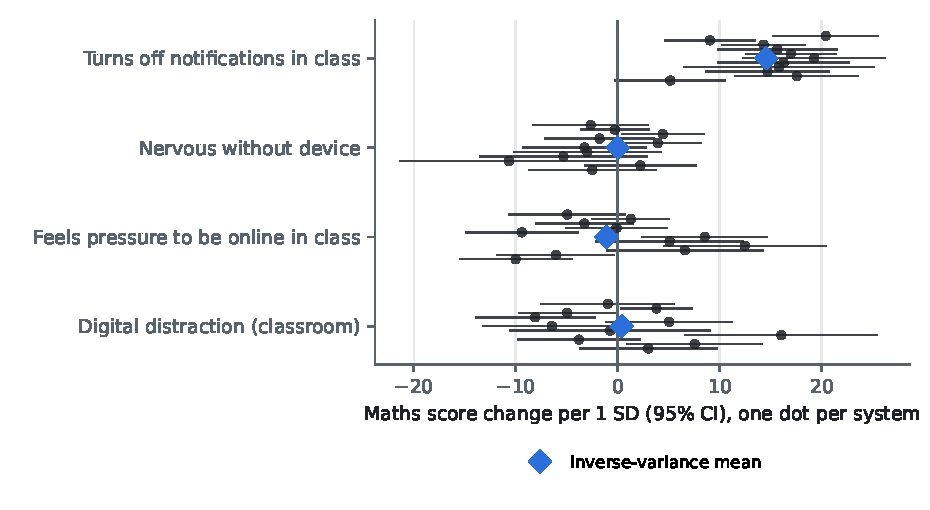
\includegraphics[width=\textwidth]{Fig4_digital_habits_math.pdf}
\caption{Digital habits and mathematics in eleven computer-based systems. Dots and bars: coefficients and 95\% BRR/Rubin intervals from all ten plausible values; blue diamonds: inverse-variance means. Final weights and model-specific complete cases; total analytic $n=13,339$, with system counts in Table~\ref{tab:modeln} (M4).}\label{fig:habits}
\end{figure}

\subsection{School phone policies (H5)}
Only 11.6\% of Vietnamese students attended schools whose principal reported that phones were not allowed on the premises, compared with 64--81\% in Hong Kong, Malaysia and Brunei (Table~\ref{tab:policyprev}). In the naive pooled model, bans were associated with less distraction and with lower mathematics scores (Table~\ref{tab:policymodels}). After inverse-probability weighting (Table~\ref{tab:ipw}), bans remained associated with less distraction ($-0.08$ SD, $p<.001$), whereas the achievement difference shrank to $-1.9$ points and was not significant. The attenuation is consistent with measured selection into bans; residual confounding and uncertainty prevent a causal interpretation. Bans were not associated with anxiety. Responsible-internet programmes were associated with lower anxiety in the pooled model, and in Viet Nam with less distraction. The phone-ban part of H5 is consistent with the distraction association; the self-regulation part is consistent with the achievement associations in the computer-based systems. Neither is a causal policy estimate.

\begin{table}[H]\centering\footnotesize
\caption{Students in schools with each device policy, PISA 2022 (\%)}\label{tab:policyprev}
\begin{tabular}{@{}lrrrr@{}}
\toprule
System & Phone ban & Co-created rules & Responsible-internet & SEL policy \\
 & (\% students) & (\%) & programme (\%) & (\%) \\
\midrule
\textbf{Viet Nam} & 11.7 & 78.7 & 70.8 & 66.1 \\
Singapore & 15.5 & 88.4 & 99.4 & 98.7 \\
Japan & 38.1 & 55.9 & 57.2 & -- \\
Korea & 23.3 & 83.5 & 77.7 & 73.5 \\
Chinese Taipei & 45.8 & 77.5 & 68.1 & 44.2 \\
Hong Kong (China) & 67.0 & 59.8 & 86.3 & 60.9 \\
Macao (China) & 46.3 & 50.8 & 83.2 & 70.7 \\
Thailand & 12.4 & 90.1 & 57.9 & 85.0 \\
Malaysia & 64.4 & 60.2 & 61.2 & 70.0 \\
Indonesia & 43.5 & 85.4 & 76.7 & 79.0 \\
Philippines & 30.0 & 94.3 & 77.8 & 86.1 \\
Brunei Darussalam & 80.9 & 91.0 & 59.4 & 40.9 \\
Cambodia & 33.4 & 73.1 & 66.3 & 62.0 \\
\bottomrule
\end{tabular}

\end{table}

\begin{table}[H]\centering\scriptsize
\caption{School policies and student outcomes, regression adjustment (SE in parentheses)}\label{tab:policymodels}
\begin{tabular}{@{}lrrrrrr@{}}
\toprule
 & \multicolumn{3}{c}{Pooled, 13 systems (system FE)} & \multicolumn{3}{c}{Viet Nam} \\
School policy & Distraction & Anxiety & Maths & Distraction & Anxiety & Maths \\
\midrule
Phones not allowed on premises & -0.11*** (0.01) & 0.00 (0.01) & -4.9* (1.9) & -0.04 (0.05) & -0.08 (0.05) & -9.2 (6.9) \\
Rules co-created with students & -0.03 (0.02) & -0.01 (0.02) & -0.7 (2.1) & -0.01 (0.04) & -0.11* (0.05) & -2.5 (6.9) \\
Responsible-internet programme & -0.03 (0.02) & -0.05* (0.02) & 2.4 (2.3) & -0.11* (0.05) & 0.01 (0.03) & -0.1 (7.5) \\
SEL policy & 0.00 (0.02) & 0.01 (0.02) & 0.3 (2.3) & -0.03 (0.05) & -0.02 (0.04) & -1.0 (6.6) \\
\bottomrule
\end{tabular}

\par\smallskip\raggedright\footnotesize Controls: student ESCS, school-mean ESCS, gender, grade, urban location; anxiety and mathematics models also control for DIGDIST. Singapore programme estimates rest on very few schools without the programme.
\end{table}

\begin{table}[H]\centering\footnotesize
\caption{School phone bans: pooled estimates with inverse-probability weighting (13 systems, system fixed effects)}\label{tab:ipw}
\begin{tabular}{@{}lrrr@{}}
\toprule
Outcome & Unadjusted & IPW + student controls & $N$ \\
\midrule
Digital distraction (SD) & -0.082*** (0.011) & -0.084*** (0.011) & 44,589 \\
Maths anxiety (SD) & -0.017 (0.014) & -0.020 (0.013) & 53,501 \\
Mathematics (points) & -4.7 (3.0) & -1.9 (2.4) & 85,299 \\
\bottomrule
\end{tabular}

\par\smallskip\raggedright\footnotesize Propensity score from school-mean ESCS, urban location, log school size and private management, estimated within each system; propensity probabilities clipped to .05/.95 before forming the weights.
\end{table}

\section{Discussion}

\paragraph{Well-being trends and measurement (H1)} Viet Nam's rapid connectivity coincided with greater reported loneliness and a measurement-invariant increase in mathematics anxiety. The targeted partial-scalar analysis substantially attenuates the belonging contrast and still fails the invariance criterion. H1 is therefore supported by specific item trends and anxiety, rather than by a robust common latent belonging decline. Wording and response-style changes warrant caution in interpreting social exclusion.

\paragraph{Home access and equity (H2)} The within-cycle and DFL results provide little support for the measured home-access account of loneliness. Sensitivity to five weighting choices strengthens this descriptive conclusion, without ruling out intensity of use, content, reverse causation or unobserved confounding. Aggregate trends \citep{twenge2021,twenge2025} and small individual associations \citep{orben2019,vuorre2021} can coexist. An ecological mechanism remains a hypothesis to investigate. Meanwhile, the increasing adjusted home-computer achievement association raises an equity concern; repeated cross-sections cannot establish that devices caused the gap.

\paragraph{Classroom climate and emotions (H3/H4)} The distraction--achievement association attenuates after non-digital disorder is included, consistent with classroom attention and cognitive-load accounts \citep{sweller1988}. Conditioning on a concurrent climate measure does not identify mediation, because temporal ordering and confounding of mediator and outcome are unresolved. The remaining distraction--anxiety association in Viet Nam is consistent with control-value theory \citep{pekrun2006}. Cross-system significance differences do not themselves prove different effect sizes; interactions would be required for that claim. The regression reliability plots show reasonable mathematics calibration and an anxiety calibration slope below one. SHAP describes prediction under correlated features, not mechanisms or causal variable importance.

\paragraph{Phone policies and self-regulation (H5)} Bans are associated with less distraction after adjustment, while adjusted achievement and anxiety differences remain statistically uncertain. Propensity weighting addresses measured school characteristics only. Turning off notifications is positively associated with achievement in most computer-based systems, but behavioural selection may explain part of this pattern. Classroom management and self-regulation merit prospective evaluation alongside Viet Nam's conditional phone rule \citep{moet2020circular32}.

\paragraph{Pandemic and concurrent policy changes} PISA has no observations for 2020/2021 in this dataset. The loneliness increase was already 6.55 percentage points in 2012--2018, followed by 1.72 points in 2018--2022; belonging agreement decreased in the first interval but recovered in the second (Table~\ref{tab:pandemic}). Thus COVID-19 alone cannot explain the earlier item trend, but the later interval does not isolate a closure effect. OECD's PISA 2022 analysis places pandemic disruptions alongside longer-term changes \citep{oecd2023vol2}. Viet Nam also adopted the 2018 general curriculum, with grade 10 scheduled from 2022/2023, and changed national graduation/university-entry assessment from 2015 \citep{moet2018curriculum,government2015exam}. These reforms are concurrent context, not estimated causes; implementation dates and individual curriculum exposure must be checked before attributing the 2022 observations to the new grade-10 programme. Examination pressure and changing instruction remain alternative explanations.

\paragraph{Methodological contribution and recent evidence} The contribution combines multi-cycle harmonisation with measurement-invariance tests, sequential DFL decomposition, and LightGBM/SHAP tracking of predictive importance across cycles in ten East and Southeast Asian systems. This regional design should not be described as a global sample. Recent evidence includes OECD's PISA-2022 screen-time analysis \citep{oecd2024screen}, a 2024 adolescent device-use/achievement meta-analysis \citep{wang2024}, and a 2025 systematic review of digital distractions \citep{martin2025}. The latter already recognises technology, personal and environmental factors. Our addition is the joint temporal, measurement and distributional analysis of PISA data; ecological framing itself is not new. The 2024 meta-analysis is not exclusively a PISA-2022 synthesis, and the 2025 review is not a meta-analysis.

\paragraph{Implications and limitations} Monitor item-specific well-being alongside digital inclusion; evaluate classroom climate and self-regulation interventions; and prioritise equitable learning resources. These are research and policy priorities, not demonstrated treatment benefits. Repeated cross-sections, complete-case selection, coarse access measures and concurrent outcomes limit causal inference. DFL accounts for measured distributional shifts only. Belonging remains non-invariant, and weighted-moment continuous-item CFA is an approximation to ordinal responses. Predictive calibration is internal school-grouped validation, without external or prospective validation. Mathematics trends omit link error; Viet Nam's 2018 performance values are unavailable. Principal-reported policies and the small number of systems further limit inference.

\section{Conclusion}
For H1, Vietnamese students reported more loneliness and mathematics anxiety, but the partial-scalar check weakens a broad latent belonging-decline claim. For H2, measured home access does not account for the loneliness trend across reweighting specifications; its strengthening achievement association nevertheless raises an equity concern. For H3/H4, the adjusted patterns connect distraction with classroom climate and anxiety without identifying mediation. For H5, phone bans correlate with less distraction and self-regulation correlates with achievement, while causal policy effects remain unresolved. Longitudinal and intervention evidence is needed to guide a well-being and equity agenda for digital education.

\section*{Ethics statement}
The study uses publicly released, de-identified secondary data. No new data were collected and no ethical approval was required.

\section*{Data and code availability}
The international student and school files are available from the \href{https://www.oecd.org/en/data/datasets/pisa-2022-database.html}{OECD PISA database}, with earlier cycles linked in the accompanying code documentation. Context indicators come from \href{https://databank.worldbank.org/source/world-development-indicators}{World Bank WDI}, \href{https://www.who.int/data/gho}{WHO GHO} and \href{https://education-profiles.org}{UNESCO PEER}. A publication repository folder containing code, aggregate results, figure sources and LaTeX has been prepared locally for release. A public code URL/DOI has not yet been assigned and must be added before submission; individual-level data are obtained from the original providers rather than redistributed in this folder.

\section*{CRediT authorship contribution statement}
\tbd{Author 1}: Conceptualization, Methodology, Formal analysis, Writing -- original draft. \tbd{Author 2}: Validation, Writing -- review \& editing.

\section*{Declaration of competing interest}
The authors declare no competing interests.

\section*{Declaration of generative AI use}
OpenAI Codex was used to assist with programming, robustness analyses, language editing and LaTeX preparation. It was not used to generate student observations or substitute for empirical estimates. The authors are responsible for reviewing the analyses, references and final text and for the content of the submitted article.

\printbibliography

\appendix
\section{Supplementary tables and figures}
\setcounter{table}{0}\renewcommand{\thetable}{A\arabic{table}}
\setcounter{figure}{0}\renewcommand{\thefigure}{A\arabic{figure}}
\renewcommand{\theHtable}{A\arabic{table}}
\renewcommand{\theHfigure}{A\arabic{figure}}

\begin{table}[H]\centering\footnotesize
\caption{PISA administration mode by system and cycle}\label{tab:mode}
\begin{tabular}{@{}lrrrr@{}}
\toprule
System & 2012 & 2015 & 2018 & 2022 \\
\midrule
Hong Kong (China) & paper & computer & computer & computer \\
Indonesia & paper & paper & computer & computer \\
Japan & paper & computer & computer & computer \\
Korea & paper & computer & computer & computer \\
Macao (China) & paper & computer & computer & computer \\
Malaysia & paper & -- & computer & computer \\
Singapore & paper & computer & computer & computer \\
Chinese Taipei & paper & computer & computer & computer \\
Thailand & paper & computer & computer & computer \\
Viet Nam & paper & paper & paper & paper \\
\bottomrule
\end{tabular}

\end{table}

\begin{table}[H]\centering\scriptsize
\caption{Earlier diagnostic latent-mean specifications, Viet Nam (2012 SD units; invariance failed)}\label{tab:latent}
\begin{tabular}{@{}llrrr@{}}
\toprule
Scale & Model & 2015 & 2018 & 2022 \\
\midrule
Belonging & scalar & +0.18 & -0.66 & -0.25 \\
Belonging & partial scalar (free intercepts: B6) & +0.15 & -0.71 & -0.26 \\
Belonging & partial scalar (free intercepts: B5) & +0.21 & -0.70 & -0.39 \\
Belonging & partial scalar (free intercepts: B5, B2) & +0.41 & -0.92 & -0.65 \\
Belonging (excl. 2018) & scalar & +0.16 & -- & -0.25 \\
Belonging (excl. 2018) & partial scalar (free intercepts: B6) & +0.14 & -- & -0.25 \\
Belonging (excl. 2018) & partial scalar (free intercepts: B5) & +0.20 & -- & -0.38 \\
Belonging (excl. 2018) & partial scalar (free intercepts: B5, B2) & +0.37 & -- & -0.66 \\
Maths anxiety & scalar & -- & -- & +0.33 \\
\bottomrule
\end{tabular}

\par\smallskip\raggedright\footnotesize Earlier belonging specifications are shown for comparison and do not validate latent trends. The targeted negative-item analysis in Tables~\ref{tab:partial}--\ref{tab:partialmeans} supersedes any claim of a substantial robust decline.
\end{table}

\begin{table}[H]\centering\footnotesize
\caption{Out-of-sample $R^2$ (school-grouped five-fold CV), PISA 2022}\label{tab:ml}
\begin{tabular}{@{}lrrrr@{}}
\toprule
 & \multicolumn{2}{c}{Mathematics} & \multicolumn{2}{c}{Maths anxiety} \\
System & LightGBM & Linear & LightGBM & Linear \\
\midrule
\textbf{Viet Nam} & 0.371 & 0.301 & 0.199 & 0.197 \\
Singapore & 0.522 & 0.464 & 0.256 & 0.268 \\
Japan & 0.441 & 0.398 & 0.167 & 0.173 \\
Korea & 0.472 & 0.416 & 0.205 & 0.199 \\
Chinese Taipei & 0.524 & 0.453 & 0.213 & 0.211 \\
Hong Kong (China) & 0.393 & 0.315 & 0.297 & 0.303 \\
Macao (China) & 0.474 & 0.461 & 0.251 & 0.270 \\
Thailand & 0.393 & 0.269 & -- & -- \\
Malaysia & 0.556 & 0.471 & 0.179 & 0.183 \\
Indonesia & 0.364 & 0.248 & -- & -- \\
Philippines & 0.562 & 0.455 & -- & -- \\
Brunei Darussalam & 0.542 & 0.452 & 0.107 & 0.131 \\
Cambodia & 0.435 & 0.296 & 0.134 & 0.137 \\
\bottomrule
\end{tabular}

\end{table}

\begin{table}[H]\centering\scriptsize
\caption{System-level context, 2022 (World Bank, WHO, UNESCO PEER, PISA)}\label{tab:system}
\begin{tabular}{@{}lrrp{4.2cm}rrr@{}}
\toprule
System & Internet & GDP pc & National phone policy (PEER) & Suicide & Distracted & School ban \\
 & users (\%) & (PPP, \$k) & & rate & (\%) & (\%) \\
\midrule
\textbf{Viet Nam} & 78.6 & 13.0 & National conditional restriction & 7.3 & 14.2 & 11.7 \\
Singapore & 96.0 & 134.8 & School discretion & 8.1 & 27.3 & 15.5 \\
Japan & 84.9 & 46.8 & Not documented in PEER & 17.4 & 5.2 & 38.1 \\
Korea & 97.2 & 53.2 & School discretion & 27.5 & 9.4 & 23.3 \\
Chinese Taipei & -- & -- & Not covered by PEER & -- & 15.9 & 45.8 \\
Hong Kong (China) & 95.6 & 64.0 & School discretion & -- & 16.4 & 67.0 \\
Macao (China) & 89.5 & 59.9 & School discretion & -- & 13.3 & 46.3 \\
Thailand & 88.0 & 20.8 & School discretion & 16.6 & 26.4 & 12.4 \\
Malaysia & 97.4 & 32.1 & No national rule found & 5.7 & 20.3 & 64.4 \\
Indonesia & 66.5 & 13.3 & No national rule & 1.2 & 25.1 & 43.5 \\
Philippines & 75.2 & 9.5 & No national rule found & 3.5 & 40.9 & 30.0 \\
Brunei Darussalam & 99.0 & 76.4 & National ban (bringing phones to school) & 3.0 & 11.5 & 80.9 \\
Cambodia & 65.5 & 6.5 & School discretion & 4.5 & 19.2 & 33.4 \\
\bottomrule
\end{tabular}

\par\smallskip\raggedright\footnotesize Suicide rate: per 100,000, both sexes, all ages, 2021 (WHO). Across systems, distraction was not related to internet penetration ($\rho=-0.29$, $n=12$) or to the share of schools banning phones ($\rho=-0.28$, $n=13$). PEER coding with verbatim evidence: \texttt{data/raw/policy/peer\_phone\_policy\_coding.csv}.
\end{table}

\begin{figure}[H]\centering
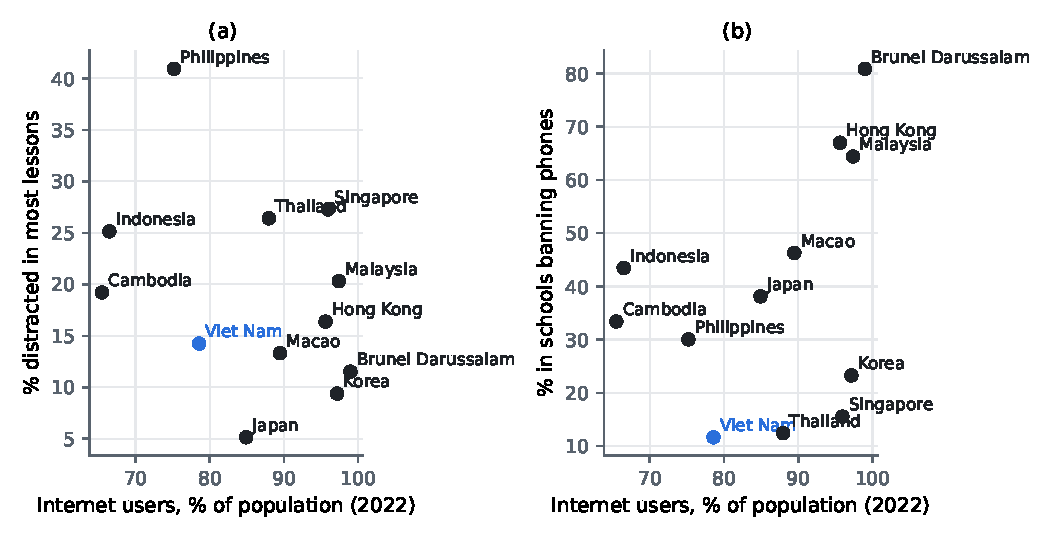
\includegraphics[width=\textwidth]{FigS1_system_scatter.pdf}
\caption{System context: (a) internet users versus distraction; (b) internet users versus phone bans. Available systems: $n=12$ and $n=13$. Student aggregates use final weights; system points are descriptive and unweighted.}
\end{figure}

\begin{figure}[H]\centering
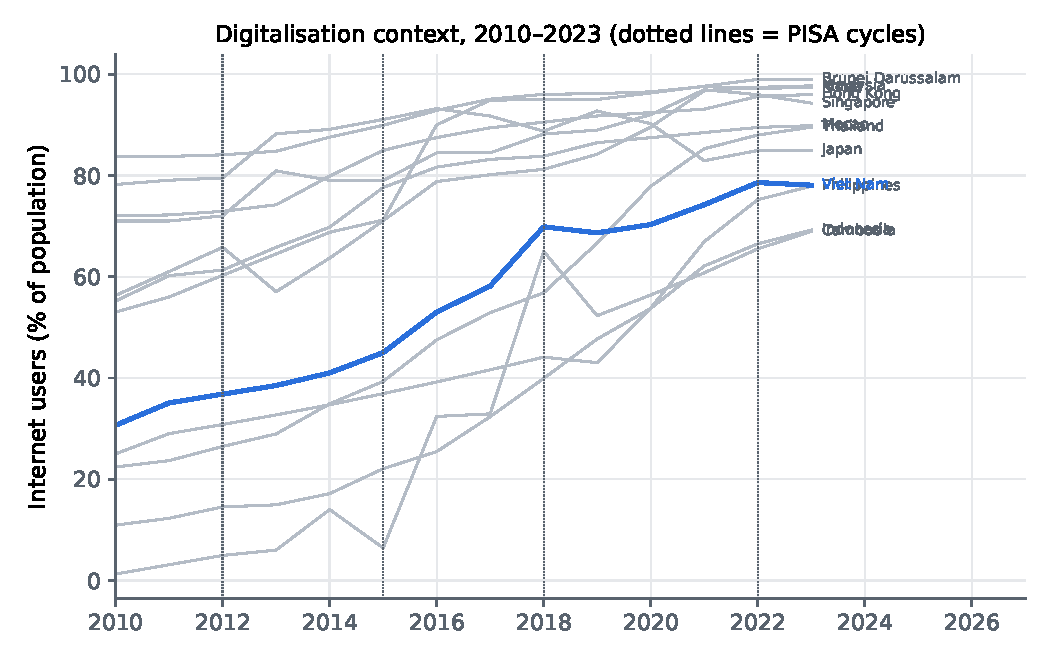
\includegraphics[width=.9\textwidth]{FigS2_internet_trajectories.pdf}
\caption{Internet users (\% of population), 2010--2023 (World Bank).}
\end{figure}
\subsection{Additional measurement, sensitivity and calibration checks}
\begin{table}[H]\centering\scriptsize
\caption{Belonging: targeted partial-scalar invariance, Viet Nam}\label{tab:partial}
\begin{tabular}{@{}llrrrrr@{}}
\toprule
Cycles & Model & $n$ & df & CFI & RMSEA & $\Delta$CFI\\
\midrule
Four & Configural & 20,213 & 24 & 0.981 & 0.052 & --\\
Four & Metric & 20,213 & 39 & 0.976 & 0.046 & --\\
Four & Scalar & 20,213 & 54 & 0.749 & 0.127 & -0.227\\
Four & Partial (negative free) & 20,213 & 45 & 0.916 & 0.080 & -0.060\\
Three & Configural & 14,920 & 18 & 0.985 & 0.048 & --\\
Three & Metric & 14,920 & 28 & 0.980 & 0.044 & --\\
Three & Scalar & 14,920 & 38 & 0.743 & 0.135 & -0.237\\
Three & Partial (negative free) & 14,920 & 32 & 0.905 & 0.089 & -0.075\\
\bottomrule
\end{tabular}
\par\smallskip\raggedright\footnotesize Final student weights; complete cases on all six items. Three-cycle models omit 2018. B3 (positive belonging) anchors the factor; B1, B4 and B6 intercepts are free across groups, with correlated residuals among these negative items. All models converged. Scalar and partial-scalar $\Delta$CFI are relative to the metric model; neither meets the $-0.010$ criterion. Weighted-moment ML treats the four response categories as continuous; fit statistics are not survey-adjusted chi-square tests.
\end{table}

\begin{table}[H]\centering\scriptsize
\caption{Belonging: sensitivity of the 2022 latent mean relative to 2012}\label{tab:partialmeans}
\begin{tabular}{@{}llr@{}}
\toprule
Cycles & Specification & 2012 SD units\\
\midrule
Four & Full scalar & -0.250\\
Four & Partial (negative free) & -0.035\\
Three & Full scalar & -0.246\\
Three & Partial (negative free) & -0.042\\
\bottomrule
\end{tabular}
\par\smallskip\raggedright\footnotesize The full-scalar specification is a diagnostic comparison and fails invariance. The targeted partial-scalar models also fail; these point estimates do not establish a common latent-mean change. No design-based confidence interval is claimed.
\end{table}

\begin{table}[H]\centering\scriptsize
\caption{Belonging: item distributions by cycle, Viet Nam}\label{tab:itemsB}
\begin{tabular}{@{}lrrrrrrrrr@{}}
\toprule
Item & Year & $n$ & Missing\% & Mean & SD & 1\% & 2\% & 3\% & 4\%\\
\midrule
B1 & 2012 & 3,301 & 33.4 & 3.26 & 0.60 & 1.6 & 4.0 & 61.7 & 32.7\\
B2 & 2012 & 3,301 & 33.4 & 3.13 & 0.55 & 0.5 & 7.5 & 69.9 & 22.0\\
B3 & 2012 & 3,281 & 33.8 & 2.98 & 0.61 & 1.2 & 16.1 & 66.2 & 16.5\\
B4 & 2012 & 3,294 & 33.6 & 3.12 & 0.62 & 1.2 & 10.1 & 63.9 & 24.8\\
B5 & 2012 & 3,299 & 33.5 & 2.36 & 0.68 & 8.2 & 50.9 & 37.5 & 3.3\\
B6 & 2012 & 3,295 & 33.6 & 3.28 & 0.60 & 1.0 & 5.2 & 59.0 & 34.9\\
B1 & 2015 & 5,796 & 0.5 & 3.51 & 0.62 & 0.9 & 3.7 & 39.1 & 56.3\\
B2 & 2015 & 5,803 & 0.4 & 3.17 & 0.60 & 1.4 & 6.9 & 65.1 & 26.6\\
B3 & 2015 & 5,772 & 0.9 & 2.93 & 0.66 & 3.1 & 16.1 & 65.4 & 15.4\\
B4 & 2015 & 5,798 & 0.5 & 3.05 & 0.69 & 2.1 & 15.2 & 58.6 & 24.1\\
B5 & 2015 & 5,793 & 0.6 & 2.36 & 0.73 & 10.5 & 46.9 & 38.3 & 4.3\\
B6 & 2015 & 5,798 & 0.5 & 3.40 & 0.69 & 2.2 & 5.3 & 42.5 & 50.0\\
B1 & 2018 & 5,341 & 0.7 & 2.82 & 0.74 & 4.9 & 22.7 & 57.3 & 15.0\\
B2 & 2018 & 5,342 & 0.7 & 2.92 & 0.64 & 2.5 & 17.5 & 65.5 & 14.5\\
B3 & 2018 & 5,324 & 1.0 & 2.80 & 0.64 & 3.1 & 23.2 & 64.4 & 9.4\\
B4 & 2018 & 5,337 & 0.7 & 2.87 & 0.67 & 3.3 & 20.0 & 62.9 & 13.8\\
B5 & 2018 & 5,333 & 0.8 & 2.32 & 0.68 & 8.8 & 54.4 & 33.5 & 3.4\\
B6 & 2018 & 5,340 & 0.7 & 3.13 & 0.70 & 3.3 & 9.4 & 58.7 & 28.7\\
B1 & 2022 & 5,986 & 1.4 & 2.95 & 0.80 & 6.7 & 14.8 & 55.8 & 22.8\\
B2 & 2022 & 6,011 & 0.9 & 3.05 & 0.72 & 4.7 & 10.0 & 61.3 & 24.1\\
B3 & 2022 & 5,987 & 1.3 & 2.95 & 0.66 & 3.5 & 14.1 & 66.7 & 15.8\\
B4 & 2022 & 6,002 & 1.1 & 2.77 & 0.72 & 5.3 & 24.2 & 58.8 & 11.8\\
B5 & 2022 & 5,982 & 1.4 & 2.67 & 0.69 & 5.4 & 29.5 & 57.6 & 7.5\\
B6 & 2022 & 6,003 & 1.1 & 3.08 & 0.79 & 6.7 & 7.7 & 56.6 & 29.0\\
\bottomrule
\end{tabular}
\par\smallskip\raggedright\footnotesize Available-case means, population SDs and category percentages use final student weights; missing percentage is unweighted relative to the Vietnamese cycle sample. B1 outsider, B2 friends, B3 belonging, B4 awkward, B5 liked, B6 lonely; B1/B4/B6 are reversed, so higher B responses indicate more belonging. A1 worry about difficulty, A2 tense with homework, A3 nervous with problems, A4 helpless, A5 worry about poor grades; higher A responses indicate more anxiety. Items A1--A5 are available in 2012/2022 only. SD is dispersion, not a standard error.
\end{table}

\begin{table}[H]\centering\scriptsize
\caption{Mathematics anxiety: item distributions by cycle, Viet Nam}\label{tab:itemsA}
\begin{tabular}{@{}lrrrrrrrrr@{}}
\toprule
Item & Year & $n$ & Missing\% & Mean & SD & 1\% & 2\% & 3\% & 4\%\\
\midrule
A1 & 2012 & 3,295 & 33.6 & 2.81 & 0.67 & 2.7 & 25.2 & 60.2 & 11.9\\
A2 & 2012 & 3,260 & 34.3 & 2.27 & 0.69 & 10.1 & 56.6 & 29.3 & 4.0\\
A3 & 2012 & 3,288 & 33.7 & 2.40 & 0.72 & 8.7 & 47.6 & 38.6 & 5.1\\
A4 & 2012 & 3,290 & 33.7 & 2.34 & 0.68 & 8.2 & 52.9 & 35.1 & 3.7\\
A5 & 2012 & 3,289 & 33.7 & 2.85 & 0.80 & 6.2 & 22.3 & 52.4 & 19.2\\
A1 & 2022 & 5,938 & 2.1 & 2.91 & 0.80 & 4.9 & 21.8 & 50.7 & 22.5\\
A2 & 2022 & 5,928 & 2.3 & 2.50 & 0.81 & 7.9 & 46.6 & 33.3 & 12.2\\
A3 & 2022 & 5,908 & 2.6 & 2.54 & 0.82 & 8.1 & 42.8 & 36.1 & 13.0\\
A4 & 2022 & 5,923 & 2.4 & 2.38 & 0.82 & 10.6 & 52.6 & 25.5 & 11.3\\
A5 & 2022 & 5,924 & 2.4 & 3.05 & 0.78 & 4.8 & 13.9 & 53.2 & 28.1\\
\bottomrule
\end{tabular}
\par\smallskip\raggedright\footnotesize Available-case means, population SDs and category percentages use final student weights; missing percentage is unweighted relative to the Vietnamese cycle sample. B1 outsider, B2 friends, B3 belonging, B4 awkward, B5 liked, B6 lonely; B1/B4/B6 are reversed, so higher B responses indicate more belonging. A1 worry about difficulty, A2 tense with homework, A3 nervous with problems, A4 helpless, A5 worry about poor grades; higher A responses indicate more anxiety. Items A1--A5 are available in 2012/2022 only. SD is dispersion, not a standard error.
\end{table}

\begin{table}[H]\centering\scriptsize
\caption{DFL sensitivity to propensity and density-ratio clipping, Viet Nam}\label{tab:dflsens}
\begin{tabular}{@{}llrrr@{}}
\toprule
Outcome & Weights & Composition (SE) & Access (SE) & Residual (SE)\\
\midrule
Loneliness (pp) & Untrimmed & -0.6 (0.4) & -1.2 (1.8) & 10.1 (2.0)\\
Belonging (1--4) & Untrimmed & -0.00 (0.01) & 0.05 (0.03) & -0.16 (0.03)\\
Anxiety (1--4) & Untrimmed & -0.00 (0.01) & 0.01 (0.03) & 0.13 (0.03)\\
Tension (pp) & Untrimmed & -0.5 (0.5) & -0.5 (2.1) & 13.2 (2.5)\\
Noise (pp) & Untrimmed & -0.6 (0.5) & 1.5 (2.0) & 6.1 (2.3)\\
Loneliness (pp) & PS .01/.99 & -0.6 (0.4) & -1.2 (1.8) & 10.1 (2.0)\\
Belonging (1--4) & PS .01/.99 & -0.00 (0.01) & 0.05 (0.03) & -0.16 (0.03)\\
Anxiety (1--4) & PS .01/.99 & -0.00 (0.01) & 0.01 (0.03) & 0.13 (0.03)\\
Tension (pp) & PS .01/.99 & -0.5 (0.5) & -0.5 (2.1) & 13.2 (2.5)\\
Noise (pp) & PS .01/.99 & -0.6 (0.5) & 1.5 (2.0) & 6.1 (2.3)\\
Loneliness (pp) & PS .05/.95 & -0.6 (0.4) & -1.0 (1.3) & 9.8 (1.6)\\
Belonging (1--4) & PS .05/.95 & -0.00 (0.01) & 0.04 (0.02) & -0.15 (0.03)\\
Anxiety (1--4) & PS .05/.95 & -0.00 (0.01) & 0.00 (0.02) & 0.14 (0.03)\\
Tension (pp) & PS .05/.95 & -0.5 (0.5) & -1.6 (1.6) & 14.3 (2.1)\\
Noise (pp) & PS .05/.95 & -0.6 (0.5) & 1.3 (1.4) & 6.3 (1.8)\\
Loneliness (pp) & Ratio 1/99 pct & -0.5 (0.4) & -1.3 (1.6) & 10.0 (1.9)\\
Belonging (1--4) & Ratio 1/99 pct & -0.00 (0.01) & 0.04 (0.03) & -0.15 (0.03)\\
Anxiety (1--4) & Ratio 1/99 pct & -0.00 (0.01) & 0.01 (0.03) & 0.13 (0.03)\\
Tension (pp) & Ratio 1/99 pct & -0.5 (0.5) & -1.0 (2.0) & 13.6 (2.4)\\
Noise (pp) & Ratio 1/99 pct & -0.4 (0.4) & 1.4 (1.7) & 6.0 (2.1)\\
Loneliness (pp) & Ratio 5/95 pct & -0.0 (0.2) & -1.6 (1.1) & 9.8 (1.4)\\
Belonging (1--4) & Ratio 5/95 pct & -0.01 (0.00) & 0.04 (0.01) & -0.15 (0.02)\\
Anxiety (1--4) & Ratio 5/95 pct & 0.00 (0.00) & -0.00 (0.02) & 0.14 (0.03)\\
Tension (pp) & Ratio 5/95 pct & 0.0 (0.2) & -2.0 (1.3) & 14.2 (2.1)\\
Noise (pp) & Ratio 5/95 pct & -0.1 (0.2) & 0.6 (1.0) & 6.5 (1.4)\\
\bottomrule
\end{tabular}
\par\smallskip\raggedright\footnotesize Final student weights multiplied by sequential reweighting ratios. PS clips probabilities; ratio clipping winsorises the density ratio at empirical percentiles, without discarding observations. Composition: gender, grade, repetition, books; access adds computer/internet. Missing covariates form separate categories; outcomes use available cases. All 80 Fay BRR replicates are refitted separately in each independent cycle (160 fits per stage/specification); variances are summed across cycles. pp = percentage points. Residual is not a causal effect.
\end{table}

\begin{table}[H]\centering\scriptsize
\caption{DFL overlap and effective sample size diagnostics, 2022 cohort}\label{tab:overlap}
\begin{tabular}{@{}lrrrrrr@{}}
\toprule
Weights & Stage & $n$ & ESS & Min PS & Max PS & Outside .05/.95\%\\
\midrule
Untrimmed & 1 & 6,068 & 3789 & 0.130 & 0.726 & 0.0\\
Untrimmed & 2 & 6,068 & 367 & 0.009 & 0.977 & 17.5\\
PS .01/.99 & 1 & 6,068 & 3789 & 0.130 & 0.726 & 0.0\\
PS .01/.99 & 2 & 6,068 & 368 & 0.009 & 0.977 & 17.5\\
PS .05/.95 & 1 & 6,068 & 3789 & 0.130 & 0.726 & 0.0\\
PS .05/.95 & 2 & 6,068 & 637 & 0.009 & 0.977 & 17.5\\
Ratio 1/99 pct & 1 & 6,068 & 4013 & 0.130 & 0.726 & 0.0\\
Ratio 1/99 pct & 2 & 6,068 & 426 & 0.009 & 0.977 & 17.5\\
Ratio 5/95 pct & 1 & 6,068 & 4799 & 0.130 & 0.726 & 0.0\\
Ratio 5/95 pct & 2 & 6,068 & 1123 & 0.009 & 0.977 & 17.5\\
\bottomrule
\end{tabular}
\par\smallskip\raggedright\footnotesize Stage 1 uses composition, stage 2 adds access. ESS is $(\sum w)^2/\sum w^2$ after multiplying the final student weight by the reweighting ratio, across all 6,068 students before excluding outcome missingness. PS ranges and the outside percentage refer to original estimated probabilities; the latter is an unweighted percentage. Limited overlap can inflate uncertainty even when point estimates are stable.
\end{table}

\begin{table}[H]\centering\scriptsize
\caption{Trends before and across the pandemic interval, Viet Nam}\label{tab:pandemic}
\begin{tabular}{@{}llrrr@{}}
\toprule
Interval & Outcome & Change & SE & Per year\\
\midrule
2012--2018 & Loneliness (pp) & 6.5 & 0.9 & 1.1\\
2012--2018 & Belonging agreement (pp) & -9.0 & 1.2 & -1.5\\
2012--2018 & Belonging (1--4) & -0.21 & 0.01 & -0.04\\
2018--2022 & Loneliness (pp) & 1.7 & 0.9 & 0.4\\
2018--2022 & Belonging agreement (pp) & 8.7 & 1.1 & 2.2\\
2018--2022 & Belonging (1--4) & 0.10 & 0.01 & 0.03\\
\bottomrule
\end{tabular}
\par\smallskip\raggedright\footnotesize Final student weights and all 80 BRR replicates; independent-cycle variances are summed. PISA observations are not available in 2020/2021, so interval differences cannot identify a pandemic effect. Agreement proportions use available responses; raw scale means use the harmonised scale.
\end{table}

\begin{table}[H]\centering\scriptsize
\caption{Conditional permutation diagnostic for home access, Viet Nam}\label{tab:perm}
\begin{tabular}{@{}llrrrrrr@{}}
\toprule
Year & Outcome & Access & $n$ & Coefficient & Null mean & Null SD & $p$\\
\midrule
2012 & Loneliness (pp) & Computer & 3,058 & -1.417 & 0.079 & 1.329 & 0.285\\
2012 & Loneliness (pp) & Internet & 3,058 & 0.561 & -0.396 & 1.419 & 0.690\\
2012 & Anxiety (1--4) & Computer & 3,060 & -0.018 & 0.008 & 0.029 & 0.505\\
2012 & Anxiety (1--4) & Internet & 3,060 & -0.040 & 0.004 & 0.032 & 0.195\\
2022 & Loneliness (pp) & Computer & 5,677 & 0.160 & 0.581 & 1.126 & 0.880\\
2022 & Loneliness (pp) & Internet & 5,677 & -2.077 & 0.379 & 1.686 & 0.210\\
2022 & Anxiety (1--4) & Computer & 5,617 & 0.003 & 0.005 & 0.022 & 0.875\\
2022 & Anxiety (1--4) & Internet & 5,617 & 0.010 & 0.008 & 0.030 & 0.710\\
\bottomrule
\end{tabular}
\par\smallskip\raggedright\footnotesize Joint computer/internet labels are shuffled 199 times within gender by ESCS-quintile strata, holding outcomes and survey weights fixed. WLS controls ESCS, gender, grade, repetition and books; complete cases are used. The two-sided empirical $p$ uses an add-one correction. This diagnostic is conditional on the chosen strata and does not test absence of causal effects or replace design-based inference.
\end{table}

\begin{table}[H]\centering\scriptsize
\caption{Reading as a comparison outcome, Viet Nam, PISA 2022}\label{tab:reading}
\begin{tabular}{@{}lrrrr@{}}
\toprule
Domain & $n$ & ICT resources coefficient & SE & $p$\\
\midrule
READ & 5,982 & 17.76 & 2.36 & $<.001$\\
MATH & 5,982 & 18.17 & 2.48 & $<.001$\\
\bottomrule
\end{tabular}
\par\smallskip\raggedright\footnotesize ICTRES is standardised within system. Both outcomes use all ten plausible values, final weights, all 80 BRR replicates and Rubin combination; complete cases on ESCS, gender, grade, repetition and ICTRES. Reading is associated with ICT resources and is not a technology-unrelated negative control. Coefficients are achievement points per predictor SD.
\end{table}

\begin{table}[H]\centering\scriptsize
\caption{School-grouped out-of-fold regression calibration, Viet Nam, 2022}\label{tab:calibration}
\begin{tabular}{@{}lrrrrrr@{}}
\toprule
Outcome & $n$ & Schools & $R^2$ & RMSE & Intercept & Slope\\
\midrule
Mathematics & 6,068 & 178 & 0.371 & 68.023 & 17.494 & 0.962\\
Anxiety & 5,934 & 178 & 0.199 & 0.851 & 0.054 & 0.877\\
\bottomrule
\end{tabular}
\par\smallskip\raggedright\footnotesize Final student weights; five-fold GroupKFold keeps each school in one fold; LightGBM handles missing predictors natively and missing targets are excluded. Mathematics results average ten PV-specific diagnostics; anxiety uses the observed index. Intercept/slope come from weighted observed-on-predicted regressions (ideal 0/1), without recalibrating the validation predictions. Intercepts and RMSE use the outcome units. These diagnostics are descriptive, not design-based confidence estimates.
\end{table}

\begin{table}[H]\centering\scriptsize
\caption{Analytic samples in distraction and digital-habit figures, PISA 2022}\label{tab:modeln}
\begin{tabular}{@{}lrrrrr@{}}
\toprule
System & M1 & M2 & A1 & A2 & M4\\
\midrule
BRN & 2,461 & 2,446 & 2,273 & 2,237 & 774\\
HKG & 2,643 & 2,633 & 2,628 & 2,608 & 908\\
IDN & 6,078 & 6,020 & -- & -- & 2,476\\
JPN & 2,672 & 2,657 & 2,652 & 2,616 & 1,122\\
KHM & 4,503 & 4,493 & 4,014 & 3,887 & --\\
KOR & 2,947 & 2,939 & 2,928 & 2,917 & 1,238\\
MAC & 2,075 & 2,068 & 2,058 & 2,049 & 716\\
MYS & 3,055 & 3,019 & 2,923 & 2,861 & 876\\
PHL & 3,180 & 3,138 & -- & -- & 1,341\\
SGP & 3,128 & 3,120 & 3,118 & 3,105 & 1,426\\
TAP & 2,691 & 2,680 & 2,681 & 2,667 & 977\\
THA & 3,903 & 3,864 & -- & -- & 1,485\\
VNM & 5,913 & 5,912 & 5,811 & 5,723 & --\\
\bottomrule
\end{tabular}
\par\smallskip\raggedright\footnotesize Unweighted complete-case student counts. M1/M2/M4 model mathematics with ten plausible values; A1/A2 model anxiety. M4 includes digital habits in the computer-based systems. Dashes indicate no model for the corresponding outcome. These counts accompany the final-weighted BRR estimates.
\end{table}

\begin{figure}[H]\centering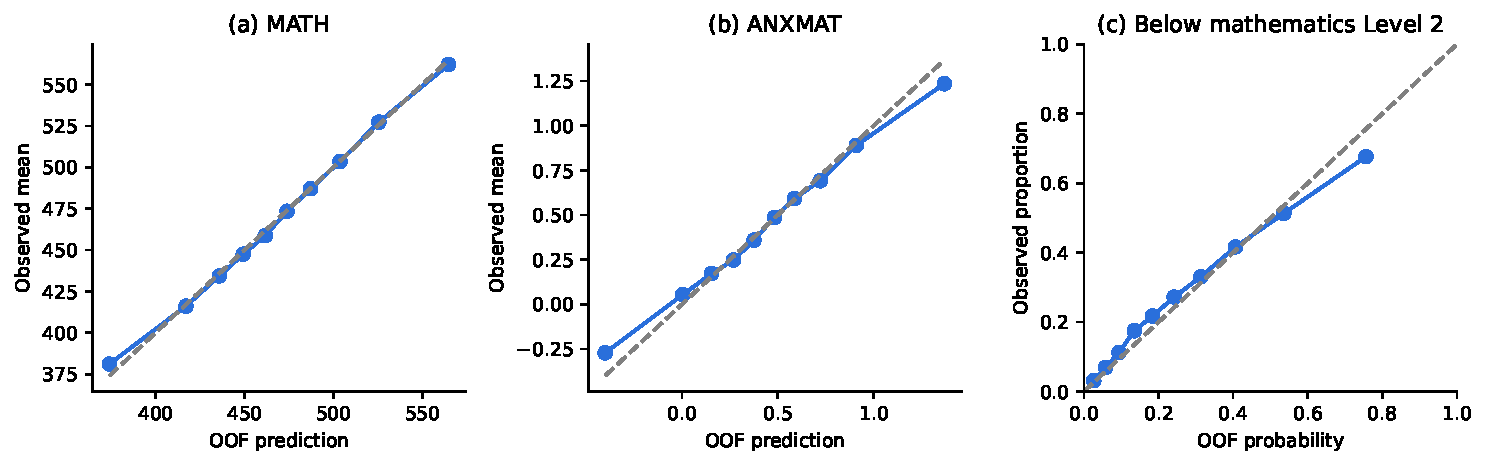
\includegraphics[width=\textwidth]{FigU_calibration.pdf}
\caption{Out-of-fold reliability, Viet Nam, PISA 2022: (a) mathematics regression ($n=6,068$, 178 schools); (b) anxiety regression ($n=5,934$, 178 schools); (c) separate classification of mathematics below Level 2, threshold 420.07 points \citep{oecd2023vol1}. Points are final-weighted means within predicted deciles; the dashed diagonal indicates perfect calibration. Mathematics panels average all ten plausible values. No confidence bands or significance tests are implied.}\label{fig:calibration}\end{figure}

The separate below-Level-2 classifiers have mean weighted Brier score 0.164, compared with 0.203 for each fold's training-prevalence baseline. Brier evaluates probabilities for this binary diagnostic, not the continuous regression. The predictions are retrospective associations using concurrent questionnaire data, not a validated prospective screening tool.

\begin{table}[H]\centering\scriptsize
\caption{Mathematics 2012--2022: link-error sensitivity in comparison systems}\label{tab:linkerror}
\begin{tabular}{@{}lrrrrr@{}}
\toprule
System & Difference & Sampling/PV SE & Link error & Total SE & 95\% interval\\
\midrule
HKG & -20.9 & 4.4 & 3.6 & 5.7 & [-32.0, -9.8]\\
IDN & -9.6 & 4.7 & 3.6 & 5.9 & [-21.1, 1.9]\\
JPN & -0.8 & 4.6 & 3.6 & 5.9 & [-12.3, 10.6]\\
KOR & -26.5 & 6.0 & 3.6 & 7.0 & [-40.1, -12.8]\\
MAC & 13.8 & 1.5 & 3.6 & 3.9 & [6.2, 21.4]\\
MYS & -11.8 & 4.0 & 3.6 & 5.4 & [-22.3, -1.3]\\
SGP & 1.2 & 1.8 & 3.6 & 4.0 & [-6.7, 9.1]\\
TAP & -12.7 & 5.0 & 3.6 & 6.2 & [-24.8, -0.7]\\
THA & -32.8 & 4.4 & 3.6 & 5.6 & [-43.9, -21.7]\\
VNM & -- & -- & -- & -- & --\\
\bottomrule
\end{tabular}
\par\smallskip\raggedright\footnotesize Student final weights; cycle means combine BRR sampling and plausible-value uncertainty. Total SE is $\sqrt{SE_{2012}^2+SE_{2022}^2+3.58^2}$, using the mathematics link error reported in NCES technical notes, Table 3 (sourced to OECD) \citep{nces2023technical}. This is a two-cycle difference, not an all-cycle trend model. Viet Nam is excluded because OECD does not establish a reliable link with its prior performance results \citep{oecd2023vnm}; adding generic link error would not repair that problem. The adjustment does not apply to questionnaire proportions or within-cycle regressions.
\end{table}

\end{document}
